% TODO L01 INTRODUCTION

\ifuniversity{tubs}{\date{October 15, 2024}}

\author{Thomas Thüm}
\lecture{Introduction}{introduction}
% goal of this lecture?
% learn what software is and distinguish term from program, software product, app, ...
% understand the importance/role of software
% understand what software engineering is good for

\inputuniversity{content/01-prelude}

\section{The Impact of Software}
% TODO several ideas illustrating impact with consequences, but then hard to distinguish from next part

\subsection{Software (Products)}
\begin{frame}{\insertsubsection}
	\begin{fancycolumns}
		\begin{definition}{Software \mysource{adapted from \sommerville}}
			Software stands for one or several computer programs and all associated documentation, libraries, support websites, and configuration data that are needed to make these programs useful.
		\end{definition}
		\begin{example}{Explanation}
			The term program is used in a broader sense here. Software may also include source code, software models, or binaries.
		\end{example}
	\nextcolumn
		\begin{definition}{Software Product and Professional Software}
			A \emph{software product} is a software that can be sold to a customer. \emph{Professional software} is software intended for use by someone apart from its developer and it is usually developed by teams rather than individuals. \mysource{adapted from \sommerville}
		\end{definition}
		\pic[width=\linewidth]{misc/ms-office-cropped}
	\end{fancycolumns}
\end{frame}

\subsection{Characteristics of Software}
\begin{frame}{\insertsubsection}
	\centering\tikz[grow cyclic,
	mindmap, every node/.style=concept,concept color=red!10!background,
	%text width=20mm,align=flush center,
	level 1/.append style={level distance=27mm,sibling angle=360/8}]
	\node {Characteristics of Software}
	child { node {abstract\\(no physical\\laws)} }
	child { node {intangible \deutsch{immateriell}} }
	child { node {hard to measure} }
	child { node {aging} }
	child { node {no \phantom{abc}deterioration} }
	child { node {no spare parts} }
	child { node {easier to adapt than hardware} }
	child { node {frequent adaptation\phantom{;}} }
	;
\end{frame}
%   abstract and intagible (immatriell): not constrained by the properties of materials, nor are they governed by physical laws or by manufacturing processes. [\sommerville]
%   good as what we can built is a matter of our imagination (and computing power)
%   bad as software can get arbitrarily complex [\sommerville]

\subsection{Application and System Software}
\begin{frame}{\insertsubsection}
	\begin{fancycolumns}[T]
		\begin{definition}{Application Software or Application}
			Software that is designed for end users and applied for certain purposes. \deutsch{Anwendungssoftware oder Anwendung}
		\end{definition}

		\begin{example}{Examples}
			web browsers, media players, email or chat clients, text or photo editors, games
		\end{example}
	\nextcolumn
		\begin{definition}{System Software}
			Software that is not application software and typically being designed to provide a platform for other software.
		\end{definition}

		\begin{example}{Examples}
			operating systems, firmware, basic input/output system (BIOS), device drivers, game engines, GUI frameworks
		\end{example}
	\end{fancycolumns}

	\uncover<3->{
		\begin{note}{Classification Not Always Unique}
			e.g., web browsers and chat clients take over more and more features of operating systems
		\end{note}
	}
\end{frame}
% mention windows being in court because IE could not be uninstalled?

\subsection{Where Does Software Run?}
\begin{frame}{\insertsubsection}
	\begin{fancycolumns}[widths={43}]
		\begin{example}{World-Wide PC Sales}
			\picDark[width=\linewidth]{history/PCsales}
		\end{example}
		\nextcolumn
		\begin{example}{World-Wide Mobile Phone Subscriptions}
			\picDark[width=\linewidth]{history/mobile-phone-subscriptions}
		\end{example}
	\end{fancycolumns}	
\end{frame}
% hardware getting smaller and smaller, portable even for bees https://www.bbc.com/news/articles/cj9jzv27lv2o

\begin{frame}{Application Software}
	\begin{fancycolumns}[T,widths={46}]
		\begin{example}{Desktop Application or Desktop App}
			Windows 1.0 released in 1985
		\end{example}
		\pic[width=\linewidth]{history/windows1.0}
	\nextcolumn
		\begin{example}{Web Application or Web App}
			Ebay was born in 1995
		\end{example}
		\pic[height=32mm]{history/flohmarkt}
		\hfill\pause
		\pic[height=32mm]{history/iPhone1stGen}
		\begin{example}{Mobile Application or Mobile App or App}
			First iPhone released in 2007
		\end{example}
	\end{fancycolumns}
\end{frame}
% history of computing/software
% * easy delivery + distribution by the internet, internet of things
% * as it is so "easy" to change software, it is changed more frequently and is typically getting more complex with every change until it dies
%		\myexample{Progressive Web Application}{since 2016, not yet popular}
% "The "brain" [computer] may one day come down to our level [of the common people] and help with our income-tax and book-keeping calculations. But this is speculation and there is no sign of it so far." 1949 Quelle "Tutorial Guide to the EDSAC Simulator" (PDF). The EDSAC Replica Project.
%  ENIAC which became operational in 1946 could be run by a single, albeit highly trained, person.

\xkcdframe{2212}
% cash vs credit/debit card vs paypal/mobile phone: more and more software involved

\subsection{Downloads of Android Apps}
\begin{frame}{Android Apps with 5 Billion Downloads \deutschertitel{5 Milliarden}}
	\centering\picDark[height=65mm]{diagrams/android-downloads-5b}
\end{frame}

\begin{frame}{Non-Preinstalled Android Apps with 5 Billion Downloads \deutschertitel{5 Milliarden}}
	\centering\picDark[height=65mm]{diagrams/android-downloads-5b-np}
\end{frame}
% TODO add facebook,whatsapp,instagram outtage from October 2021?

%\begin{frame}{Android Apps with 1 Billion Downloads \deutschertitel{1 Milliarde}}
%	\centering\picDark[height=65mm]{diagrams/android-downloads-1b-p}
%\end{frame}

%\begin{frame}{Non-Preinstalled Android Apps with 1 Billion Downloads \deutschertitel{1 Milliarde}}
%	\centering\picDark[height=65mm]{diagrams/android-downloads-1b-np}
%\end{frame}

%\begin{frame}{Android Apps with 500 Million Downloads}
%	\centering\picDark[height=65mm]{diagrams/android-downloads-500m-np}
%\end{frame}

\subsection{Categories of Software}
\begin{frame}{\insertsubsection}
	\centering\tikz[grow cyclic,
	mindmap, every node/.style=concept,concept color=blue!10!background,
	%text width=20mm,align=flush center,
	level 1/.append style={level distance=27mm,sibling angle=360/8}]
	\node {Categories of Software}
	child { node {system vs\phantom{;} application software\phantom{ab}} }
	child { node {generic vs customized} }
	child { node {proprietary\\vs open-source} }
	child { node {freeware\\vs commercial} }
	child { node {data-intensive vs computation-intensive} }
	child { node {monolithic vs distributed} }
	child { node {stand-alone vs integrated} }
	child { node {user interface vs API\phantom{ab}} }
	;
\end{frame}
% TODO parts of this diagram not readible

% software is eating the world: https://a16z.com/2011/08/20/why-software-is-eating-the-world/
% data is the new oil

% German E rezept is facing technical challenges



\lessonslearned{
	\item What is software?
	\item What is the difference between program, software product, professional software, desktop/web/mobile app?
	\item What are characteristics and properties of software?
	\item What is the impact of software?
	\item Next: What can go possibly wrong with software?
}{
	\item \sommerville\mychapter{1.1}\mypages{19--28} % TODO check
}{
	\begin{enumerate}
		\item<+-> Form groups of 2-3 students
		\item<+-> Introduce yourselves to each other (5 min)
		\item<+-> Share your (recent) experiences with software (5 min)
		\item<+-> Survey: What is your experience with software?\\
		\slideonly{~
			\item<+->[A] Warst du jemals von einer Softwarepanne betroffen?
			\item<+->[B] Hast du dich im letzten Semester über Softwarefehler geärgert?
			\item<+->[C] Hast du selbst Programmiererfahrung?
			\item<+->[D] Hast du bereits Software getestet?
			\item<+->[E] Hast du schon mal Programmierfehler verursacht?
		}
			%\fancyqr{https://studip.tu-braunschweig.de/dispatch.php/questionnaire/answer/dc864612bd163af167a09edabdf058f3?cid=c37620ed3e63513af37fbe31060fcf69&range_type=course&range_id=c37620ed3e63513af37fbe31060fcf69}
	\end{enumerate}
}

\section{Software and Its Engineering}
% Why is Engineering Good Software so Hard?
% How to Develop Good Software?
% Why is Software Production so hard?
\subsection{The Project Cartoon}
\begin{frame}[b]{\insertsubsection}
	\vspace{-20mm}\small\renewcommand{\projectcartoonwidth}{.18}
	\begin{fancycolumns}[widths={30},animation=none]
		\uncover<11->{\begin{definition}{Why Do Software Projects Fail?}
			\begin{itemize}
				\item many stakeholders with different background each
				\item miscommunication
				\item implicit or wrong assumptions
				\item time pressure
				\item high complexity
				\item \ldots
				\item numerous reasons specific to certain phases and roles
			\end{itemize}
		\end{definition}}
		\uncover<12->{\begin{note}{}\centering{}software engineering aims to\\reduce such problems\end{note}}
	\nextcolumn
		\centering\hprojectcartoon{01}{how the customer explained it} % se02-10 requirements
		\uncover<2->{\hprojectcartoon{02}{how the project leader understood it}} % se02-07 modeling
		\uncover<3->{\hprojectcartoon{03}{how the analyst designed it}} % se04-10 architecture anddesign
		\uncover<4->{\hprojectcartoon{04}{how the programmer implemented it}} % se02-10 implementation
		\uncover<5->{\hprojectcartoon{05}{what the beta testers received}} % se08-09 testing
	
		\uncover<6->{\hprojectcartoon{06}{how the business consultant described it}} % se02-03 process
		\uncover<7->{\hprojectcartoon{09}{how the customer was billed}} % se10 management and pricing
		\uncover<8->{\hprojectcartoon{10}{how it was supported}} % se12 maintenance
		\uncover<9->{\hprojectcartoon{12}{when it was delivered}} % se13 continous integration/delivery
		\uncover<10->{\hprojectcartoon{13}{what the customer really needed}} % se02-05
		%\hspace{-7mm}
		%\projectcartoon{07}{how the project was documented} % code documentation
		%\hprojectcartoon{18}{how patches were applied} % se11 evolution
		%\hprojectcartoon{17}{how it performed under load} % se14 compilation/quality assurance/performance
		%\hprojectcartoon{11}{what marketing advertised} % se15 reuse/product lines
		%\hprojectcartoon{16}{how open source version} % se16 open source/licensing
		%\projectcartoon{08}{what operations installed} % devops?
		%\projectcartoon{14}{what the digg effect can do to your site} % micro services?
		%\projectcartoon{15}{the disaster recover plan}
		%\hspace{-7mm}
	\end{fancycolumns}
\end{frame}

\subsection{Software Engineering}
\begin{frame}{\insertsubsection}
	\begin{fancycolumns}
		\begin{definition}{Software Engineering \mysource{\sommerville}}
			\mycite{Software engineering is an engineering discipline that is concerned with all aspects of software production from initial conception to operation and maintenance. [...] Software engineering is not just concerned with the technical processes of software development. It also includes activities such as software project management and the development of tools, methods, and theories to support software development.}
		\end{definition}
	\end{fancycolumns}
\end{frame}

%\subsection{Software Engineering vs Programming}
\begin{frame}[b]{Software Engineering vs Programming}
	\slideSEvsProgramming
\end{frame}

\xkcdframe{2021}

%\subsection{}
\begin{frame}{Software Engineering vs Computer Science}
	\begin{fancycolumns}[animation=none]
		\begin{definition}{SE vs CS \mysource{\sommerville}}
			\mycite{Computer science focuses on theory and fundamentals; software engineering is concerned with the practicalities of developing and delivering useful software. [...] Computer science theory, however, is often most applicable to relatively small programs. Elegant theories of computer science are rarely relevant to large, complex problems that require a software solution.}
		\end{definition}
	\nextcolumn
	\end{fancycolumns}
\end{frame}
% add picture illustrating other related areas

\subsection{Software and System Engineering}
\begin{frame}{\insertsubsection}
	\begin{fancycolumns}[animation=none]
		\begin{definition}{System Engineering \mysource{\sommerville}}
			\mycite{System engineering is concerned with all aspects of computer-based systems development including hardware, software and process engineering. Software engineering is part of this more general process.}
		\end{definition}
	\nextcolumn
		% "System engineering is therefore concerned with hardware development, policy and process design, and system deployment, as well as software engineering." [\sommerville]
		\pic[width=\linewidth]{misc/lawn-mower-cropped} % copied to process lecture
	\end{fancycolumns}
\end{frame}

\subsection{(Software) Engineering}
\begin{frame}{\insertsubsection}
	\begin{fancycolumns}[animation=none]
		\begin{definition}{Engineering \mysource{\sommerville}}
			\mycite{Engineering is about getting results of the required \emph{quality} within \emph{schedule} and \emph{budget}. [...] Engineers make things work. They apply theories, methods, and tools where these are appropriate. However, they use them selectively and always try to discover solutions to problems even when there are no applicable theories and methods. Engineers also recognize that they must work within organizational and financial constraints, and they must look for solutions within these constraints.}
		\end{definition}
		\nextcolumn
			%\posthandout{\pic[width=\linewidth,trim={0\width} {.25\height} {0\width} {.1\height},clip]{blackboard/spannungsdreieck_240408}} % TODO check blackboard
	\end{fancycolumns}
\end{frame}

% TODO in lecture: Magisches Dreieck aufmalen: cost, time, quality

\subsection{Relevance of Software for This Course}
\begin{frame}{\insertsubsection}
	\begin{exampletight}{}
		\picDark[width=\linewidth]{failures/google-scholar2}
	\end{exampletight}
\end{frame}

\begin{frame}{\insertsubsection}
	\centering\picDark[height=\textheightwithtitle]{failures/texstudio}
\end{frame}

\begin{frame}{\insertsubsection}
	\begin{fancycolumns}[widths={54},animation=none]
		\pic[width=\linewidth]{failures/obs-freeze}
	\nextcolumn
		\pic[width=\linewidth]{failures/obs-freeze2}
	\end{fancycolumns}
\end{frame}

\begin{frame}{\insertsubsection}
	\begin{fancycolumns}
		\pic[width=\linewidth]{failures/acrobat-correct-green}
		\nextcolumn
		\pic[width=\linewidth]{failures/acrobat-wrong-green}
	\end{fancycolumns}
\end{frame}

\xkcdframe{1197}

\begin{frame}{\insertsubsection}
	\centering\pic[height=\textheightwithtitle]{failures/flash}
\end{frame}

\begin{frame}{\insertsubsection}
	\centering\pic[height=\textheightwithtitle]{failures/thunderbird}
\end{frame}


\lessonslearned{
	\item What is software engineering?
	\item Which trade-off is crucial to software engineering?
	\item Next: What is expected from you during this term?
}{
	\item \sommerville\mychapter{1.1}\mypages{19--28} % TODO check
}{
	\begin{enumerate}
		\item<+-> Form groups of 2-3 students
		\item<+-> Discuss: What will you do for a living in 10 years? What will be your connection to software? (5 min)
		\item<+-> Survey: What is your connection to software in 10 years?
		\slideonly{~
			\item<+->[A] Wirst du in 10 Jahren Software entwickeln?
			\item<+->[B] Wirst du in 10 Jahren Software testen?
			\item<+->[C] Wirst du in 10 Jahren Software beauftragen?
			\item<+->[D] Wirst du in 10 Jahren Softwareanforderungen ermitteln?
			\item<+->[E] Wirst du in 10 Jahren die Entwicklung von Software leiten?
		}
	\end{enumerate}
}

\section{Course Overview}
\subsection{What You Should Know}

\begin{frame}{\myframetitle{}}
	\begin{fancycolumns}
%		\begin{note}{Fundamentals of Software Engineering}
%			\begin{itemize}
%				\item development processes
%				\item object-oriented programming
%				\item design patterns
%				\item UML class diagrams
%				\item modularity
%			\end{itemize}
%			\ifuniversity{magdeburg}{$\Rightarrow$ \emph{Software Engineering}}
%		\end{note}
	\nextcolumn
%		\begin{note}{Fundamentals of Theoretical Computer Science}
%			\begin{itemize}
%				\item set theory
%				\item propositional logic
%				\item complexity theory
%			\end{itemize}
%			\ifuniversity{magdeburg}{
%				$\Rightarrow$ \emph{Logik}\\
%				$\Rightarrow$ \emph{Grundlagen der Theoretischen Informatik I}
%			}
%		\end{note}
%		\begin{note}{Exercise}
%			solid programming skills in Java
%
%			\ifuniversity{magdeburg}{
%				$\Rightarrow$ \emph{Einführung in die Informatik}\\
%				$\Rightarrow$ \emph{Algorithmen und Datenstrukturen}
%			}
%		\end{note}
	\end{fancycolumns}
\end{frame}

\subsection{What You Will Learn}

\begin{frame}{\myframetitle{}}
	\lectureseriesoverview[1]
\end{frame}

\subsection{What You Might Need}

\begin{frame}{\myframetitle{}}
%	\myframeicon{\mytitlesource{\fospl, \featureide}}
%	\begin{fancycolumns}
%		\begin{exampletight}{Recommended Literature for Lecture \& Exercise}
%			\centering
%			\parbox{0.49\linewidth}{
%				\centering
%				\pic[width=\linewidth]{cover-fospl}
%				\emph{theory-focused}
%			}
%			\parbox{0.475\linewidth}{
%				\centering
%				\pic[width=\linewidth]{cover-featureide}
%				\emph{practice-oriented}
%			}
%		\end{exampletight}
%	\nextcolumn
%		\begin{exampletight}{Recommended Tool Support for the Exercise}
%			\centering
%			\picDark[width=\linewidth]{featureide-feature-model-editor}\\[.5ex]
%			\pic[width=0.25\linewidth]{featureide-logo}
%		\end{exampletight}
%	\end{fancycolumns}
\end{frame}

%\subsection{Credit for the Slides}
%
%\begin{frame}{\myframetitle{}}
%	\ifuniversity{anonymous}{\mynote{}{\centering\huge Anonymous Authors}}
%	\unlessuniversity{anonymous}{
%		\myframeicon{\href{https://github.com/SoftVarE-Group/Course-on-Software-Product-Lines}{\pic[scale=.75]{cc-by-sa}}}
%	}
%	\begin{fancycolumns}[columns=3,animation=none]
%	\nextcolumn
%		\unlessuniversity{anonymous}{
%			\begin{note}{Thomas Thüm}
%				\centering
%				\href{https://www.uni-ulm.de/en/in/sp/team/thuem/}{\adjincludegraphics[height=.45\textheight,trim={.125\width} 0 {.125\width} 0,clip]{thomas-thuem}}
%
%				\small Professor at Paderborn University
%
%				software engineering
%
%				FeatureIDE team leader
%			\end{note}
%		}
%	\nextcolumn
%	\end{fancycolumns}
%\end{frame}

\inputuniversity{content/01c-course}
\lessonslearned{
	\item How is this course organized?
	\item Next Lecture: Why do programming languages matter?
}{
	\item Main Book: \sommervillelink{Ian Sommerville. Software Engineering, 10. Edition, Pearson, 2018.}
}{
	\begin{itemize}
		\item Any questions?
	\end{itemize}
}

%\faq{
%	\item
%}{
%	\item
%}{
%	\item
%}

% TODO L02 IMPLEMENTATION

\ifuniversity{tubs}{\date{October 22, 2024}}

\author{Thomas Thüm}
\lecture{Implementation}{implementation}

\begin{frame}{\insertsubtitle}
	\alt<2->{
		\projectcartoon{01}{how the customer explained it}
		\projectcartoon{02}{how the project leader understood it}
		\projectcartoon{03}{how the analyst designed it} % architecture/design
	}{%
		\hprojectcartoon{01}{how the customer explained it}
		\hprojectcartoon{02}{how the project leader understood it}
		\hprojectcartoon{03}{how the analyst designed it} % architecture/design
	}%
	\hprojectcartoon{04}{how the programmer implemented it}
	%\hprojectcartoon{05}{what the beta testers received} % testing
	%\hprojectcartoon{06}{how the business consultant described it}
	%\hprojectcartoon{07}{how the project was documented} % code documentation
	%\hprojectcartoon{08}{what operations installed} % devops/continuous integration
	%\hprojectcartoon{09}{how the customer was billed} % pricing
	%\hprojectcartoon{10}{how it was supported}
	%\hprojectcartoon{11}{what marketing advertised}
	%\hprojectcartoon{12}{when it was delivered} % continous delivery
	\uncover<-0|handout:0>{\projectcartoon{13}{what the customer really needed}}
	%\hprojectcartoon{14}{what the digg effect can do to your site} % ???
	%\hprojectcartoon{15}{the disaster recover plan}
	%\hprojectcartoon{16}{how open source version} % open source/licensing
	%\hprojectcartoon{17}{how it performed under load} % quality assurance/performance
	%\hprojectcartoon{18}{how patches were applied} % software maintenance
\end{frame}

\section{Choosing a Programming Language}
\subsection{History of Programming Languages}
\begin{frame}{\insertsubsection}
	\begin{fancycolumns}
		\begin{note}{Milestones\mysource{\jonesbestpractice}}
			\begin{itemize}
				\setlength\itemsep{.1em}
				\item controlling behavior of mechanical devices by wiring or with punchcards \deutsch{Lochkarten}
				\item machine languages used during World War II
				\uncover<2->{
					\item assembly languages: distinction between human-readable instructions (source code) and executable instructions (object code)
					\item birth of compilers and interpreters having a one-to-many mapping between source and object code (opposed to one-to-one mapping in assemblers)
				}
				\uncover<3->{
					\item structured programming pioneered by David Parnas and Edsger Dijkstra
					\item high-level programming languages: high number of executable instructions for each human-readable instruction
					\item domain-specific languages, later general-purpose programming languages
				}
			\end{itemize}
		\end{note}
	\nextcolumn
		\uncover<4->{
		\begin{example}{Languages\mysource{\jonesbestpractice\ + \handbuch}}
			\begin{itemize}
				\setlength\itemsep{.1em}
				\item 1945: first high-level language Plankalkül by Konrad Zuse (compiler written in 1998)
				\item 1954: first professional high-level language FORTRAN (Formula Translator) by IBM
				\item 1963: Basic as general-purpose language
				\uncover<5->{
					\item 1959: functional language Lisp
					\item 1970: first object-oriented lang.\ Smalltalk-80
					\item 1970: declarative language SQL
				}
				\uncover<6->{
					\item 1971: Pascal by Niklaus Wirth for teaching
					\item 1974: very common procedural language C
					\item 1977: logical language Prolog
				}
				\uncover<7->{
					\item 1980: C++ as object-oriented extension of C
					\item 1990: object-oriented language Java
					\item 1990: functional language Haskell
				}
				\uncover<8->{
					\item 1991: multi-paradigm language Python (today's default for machine learning)
					\item 1995: scripting language JavaScript (web apps)
				}
			\end{itemize}
		\end{example}
	}
	\end{fancycolumns}
\end{frame}
% TODO revise and talk about paradigms and their languages

\subsection{Programming Languages Today}
\begin{frame}{\insertsubsection}
	\slideProgrammingLanguagesToday
\end{frame}

\subsection{Choice of Programming Languages}
\begin{frame}{\insertsubsection}
	\begin{fancycolumns}
		\begin{definition}{{Desired Properties\mysource{\ludewiglichter}}}
			\begin{itemize}
				\item modular implementation
				\item separation of inferfaces and implementations
				\item type system: strongly/weakly typed languages
				\item readable syntax (FORTRAN vs ALGOL60) % designed for fewer characters vs readability
				\item automatic pointer management (C vs Java)
				\item exception handling
			\end{itemize}
		\end{definition}
	\nextcolumn
		\begin{example}{Criteria in Practice}
			\begin{itemize}
				\item language required by the company or customer?
				\item existing infrastructure?
				\item domain-specific languages available?
				\item language known/liked by developers?
				\item available libraries?
				\item available tool support?
				\item language popularity?
				\item what may change in the future?
			\end{itemize}
		\end{example}
	\end{fancycolumns}
\end{frame}

\subsection{Popularity of Programming Languages}
\begin{frame}{\insertsubsection}
	\slideTiobeDiagram
\end{frame}
\begin{frame}{\insertsubsection}
	\slideTiobeTable
\end{frame}

\begin{frame}
	\begin{fancycolumns}[height=8.5cm]
		\pic[width=\linewidth,trim=0 20 0 20,clip]{people/patrick-mckenzie}
		\vspace{-7mm}
		
		\mynote{Patrick McKenzie \mysource{\href{https://twitter.com/CodeWisdom/status/1182702520696803329}{twitter.com}}}{\mycite{Every great developer you know got there by solving problems they were unqualified to solve until they actually did it.}}
		% computer scientist, entrepreneur, influencer
	\nextcolumn
		\pic[width=\linewidth,trim=0 55 0 10,clip]{people/bill-gates}
		\vspace{-7mm}
		
		\mynote{Bill Gates \mysource{\href{https://code.org/quotes}{code.org}}}{\mycite{Learning to write programs stretches your mind, and helps you think better, creates a way of thinking about things that I think is helpful in all domains.}}
		% richest person in 15 years between 1994 and 2014
	\end{fancycolumns}
\end{frame}

\subsection{Computer-Aided Software Engineering}
\begin{frame}{\insertsubsection}
	\begin{fancycolumns}[widths={55}]
		\begin{definition}{Terms \mysource{adapted from \ghezzi}}
			A \emph{tool} is an application that supports a particular activity. An \emph{environment} is a collection of related tools. Tools and environments aim at automating some of the activities that are involved in software engineering. The generic term for this field of study is \emph{computer-aided software engineering}.
		\end{definition}
	\end{fancycolumns}
\end{frame}

\widexkcdframe{378} % real programmers

\subsection{Overview on Development Tools}
\begin{frame}{\insertsubsection}
	\begin{fancycolumns}[widths={57}]
		\begin{note}{Variety of Tools \mysource{\ghezzi}}
			\begin{itemize}
				\item text(ual) editors: emacs, vim, ed, Word, \ldots
				\item graphical editors: UML editors, Powerpoint, \ldots
				\item assembler, compiler, interpreter
				\uncover<2->{
					\item configuration management tools: git, SVN, CVS, \ldots
					\item tracking tools (issue trackers): Github, Gitlab, \ldots
					\item tools for code navigation and refactoring
					\item tools for test specification, generation, execution, reporting
					\item tools for static and dynamic code analysis (e.g., debugger), reverse/reengineering, project management
				}
				\uncover<3->{
					\item integrated development environments (IDEs): Eclipse, Visual Studio, IntelliJ, Android Studio
				}
			\end{itemize}
		\end{note}
	\end{fancycolumns}
\end{frame}

%\subsection{Demo on Tool Support in Eclipse}
%\begin{frame}{\insertsubsection\ \mytitlesource{\href{https://youtu.be/Jxt77kTbFZ0?si=oGjCcdfji7NMmbM7&t=3318}{youtube.de}}}
%	\centering\pic[width=.7\linewidth,trim=0 76 0 76,clip]{demo/livecoding2} % TODO update picture to recent version
%\end{frame}

\lessonslearned{
	\item Historical perspective on programming
	\item Criteria for choosing languages
	\item Popularity of programming languages
	\item Next: What has programming to do with reading?
}{
	\item \jonesbestpractice\mychapter{8 Programming and Code Development}
	\item \handbuch\mychapter{2.4 Programming Languages}
}{
	\begin{enumerate}
		\item Enter 1+2*3 into the calculator app of your mobile device or laptop
		\item Compare the results with your colleagues
		\item Discuss why results (could) differ
	\end{enumerate}
}

\begin{frame}{Calc on Windows 10\ \mytitlesource{\href{https://youtu.be/LKDbQfzzGJo?t=1544}{youtube.de}}}
	\begin{fancycolumns}
		\centering\picDark[width=.66\linewidth]{failures/win10-calc-scientific}
	\nextcolumn
		\centering\picDark[width=.66\linewidth]{failures/win10-calc-standard}
	\end{fancycolumns}
\end{frame}

\section{Coding Conventions}
\begin{frame}
	\begin{fancycolumns}[height=8.5cm]
		\pic[width=\linewidth,trim=40 0 100 0,clip]{people/douglas-crockford}
		\vspace{-7mm}
		
		\begin{note}{Douglas Crockford \mysource{\javascript}}
			\mycite{It turns out that style matters in programming for the same reason that it matters in writing. It makes for better reading.}
		\end{note}
		% known for JavaScript, JSON, works at Paypal
	\nextcolumn
		\pic[width=\linewidth,trim=0 20 0 25,clip]{people/francois-chollet}
		\vspace{-7mm}[height=8.5cm]
		
		\begin{note}{François Chollet \mysource{\href{https://twitter.com/fchollet/status/1038200379605798912}{twitter.com}}}
			\mycite{In software, naming matters, because names reflect how you think about a problem. Code is also communication, and naming is a big part of making it work.}
		\end{note}
		% AI researcher at Google
	\end{fancycolumns}
\end{frame}

\xkcdframe{2021}

\subsection{Code Formatting}
\begin{frame}{\insertsubsection}
	\begin{fancycolumns}
		\begin{note}{Motivation}
			\begin{itemize}
				\item code is read much more often and by more developers than written
				\item avoid differences by each programmer
			\end{itemize}
		\end{note} % TODO add citation
		\begin{definition}{Code Formatting}
			\begin{itemize}
				\item indentation: typically 4 characters per level
				\item length of a line: often 80 or 100 characters
				\item extra indentation: typically 8 characters when breaking extra long lines
				\item empty lines between members (e.g., methods and attributes)
			\end{itemize}
		\end{definition} % TODO add citation
	\nextcolumn
		\begin{example}{Code Formatting in Practice}
			\begin{itemize}
				\item automated code formatters available (on demand or when saving the editor)
				\item typical formatting rules for each language
				\item automated code formatters are configurable (handle with care)
			\end{itemize}
		\end{example} % TODO add citation
	\end{fancycolumns}
\end{frame}

\subsection{Rules on Naming}
\begin{frame}{\insertsubsection}
	\begin{fancycolumns}
		\begin{example}{Unwanted Names}
			\begin{itemize}
				\item single character as a name
				\item very long names
				\item names consisting only of special chars
				\item synonyms: delete, remove, clear
				\item abbreviations (unless very common)
			\end{itemize}
		\end{example} % TODO add citation
	\nextcolumn
		\begin{definition}{Wanted Names}
			\begin{itemize}
				\item nouns for class names: Calculator
				\item nouns for attribute names: calculateButton
				\item verbs for method names: getCalculator(), evaluate(), isZero(), hasChildren(), setValue()
				\item PascalCaseNotation for classes, interfaces (not consistent in C/C++)
				\item camelCaseNotation for attributes, methods, local variables, parameters (exception: Python)
				\item UPPER\_SNAKE\_CASE\_NOTATION for constants (exception: Go)
				\item lowercasenotation for package names (exception: C\#)
			\end{itemize}
		\end{definition} % TODO add citation
	\end{fancycolumns}
\end{frame}

\begin{frame}
	\begin{fancycolumns}[height=8.5cm]
		\pic[width=\linewidth,trim=0 275 0 25,clip]{people/martin-fowler}
		\vspace{-7mm}
		
		\begin{note}{Martin Fowler (1999) \mysource{\refactoring}}
			\mycite{Any fool can write code that a computer can understand. Good programmers write code that humans can understand.}
		\end{note}
		% known for refactoring and agile development
	\nextcolumn
		\pic[width=\linewidth,trim=0 0 0 10,clip]{people/cory-house}
		\vspace{-7mm}
		
		\begin{note}{Cory House \mysource{\href{https://twitter.com/housecor/status/400479246713229312}{twitter.com}}}
			\mycite{Code is like humor. When you have to explain it, it’s bad.}
		\end{note}
		% influencer known for teaching React and JavaScript
	\end{fancycolumns}
\end{frame}

\subsection{Code Documentation}
\begin{frame}{\insertsubsection}
	\begin{fancycolumns}
		\begin{definition}{Comments \ldots}
			\begin{itemize}
				\item in source code are easier to maintain (than in external documents)
				\item should be written while editing the code
				\item can be used to generate documentation (e.g., JavaDoc, Doxygen)
				\item are used to specify classes and public methods (e.g., parameters, exceptions, dependencies)
				\item document hacks, side effects and unfinished parts (e.g., TODO)
				\item should not paraphrase the code
			\end{itemize}
		\end{definition}
	\end{fancycolumns}
\end{frame}

\begin{frame}
	\begin{fancycolumns}[height=8.5cm]
		\pic[width=\linewidth,trim=0 0 0 60,clip]{people/ryan-campbell}
		\vspace{-7mm}
		
		\begin{note}{Ryan Campbell \mysource{\href{https://handbook.problemsolving.io/01-model/03-code.html}{problemsolving.io}}}
			\mycite{Commenting your code is like cleaning your bathroom - you never want to do it, but it really does create a more pleasant experience for you and your guests.}
		\end{note}
		% software developer
	\nextcolumn
		\pic[width=\linewidth,trim=90 15 10 20,clip]{people/steve-mcconnell}
		\vspace{-7mm}
		
		\begin{note}{Steve McConnell (2004) \mysource{\codecomplete}}
			\mycite{Good code is its own best documentation. As you're about to add a comment, ask yourself, \mycite{How can I improve the code so that this comment isn't needed?} Improve the code and then document it to make it even clearer.}
		\end{note}
		% author of several textbooks on software development and project management
	\end{fancycolumns}
\end{frame}




\lessonslearned{
	\item Coding conventions \deutsch{Programmierrichtlinien}
	\item Formatting, naming, comments, and documentation
	\item Next: What tools are available for programming?
}{
	\item \javastyleguide
	% TODO add literature? \refactoring \codecomplete \javascript
}{
	\begin{enumerate}
		\item<+-> Form groups of 2-3 students
		\item What happens if each programmer applies different coding conventions? 
		\item Would it help to agree on coding conventions for each file individually?
	\end{enumerate}
}

\section{Tools and Environments}
\subsection{Computer-Aided Software Engineering}
\begin{frame}{\insertsubsection}
	\begin{fancycolumns}[widths={55}]
		\begin{definition}{Terms \mysource{adapted from \ghezzi}}
			A \emph{tool} is an application that supports a particular activity. An \emph{environment} is a collection of related tools. Tools and environments aim at automating some of the activities that are involved in software engineering. The generic term for this field of study is \emph{computer-aided software engineering}.
		\end{definition}
	\end{fancycolumns}
\end{frame}

\widexkcdframe{378} % real programmers

\subsection{Overview on Development Tools}
\begin{frame}{\insertsubsection}
	\begin{fancycolumns}[widths={57}]
		\begin{note}{Variety of Tools \mysource{\ghezzi}}
			\begin{itemize}
				\item text(ual) editors: emacs, vim, ed, Word, \ldots
				\item graphical editors: UML editors, Powerpoint, \ldots
				\item assembler, compiler, interpreter
				\uncover<2->{
				\item configuration management tools: git, SVN, CVS, \ldots
				\item tracking tools (issue trackers): Github, Gitlab, \ldots
				\item tools for code navigation and refactoring
				\item tools for test specification, generation, execution, reporting
				\item tools for static and dynamic code analysis (e.g., debugger), reverse/reengineering, project management
				}
				\uncover<3->{
				\item integrated development environments (IDEs): Eclipse, Visual Studio, IntelliJ, Android Studio
				}
			\end{itemize}
		\end{note}
	\end{fancycolumns}
\end{frame}

\subsection{Demo on Tool Support in Eclipse}
\begin{frame}{\insertsubsection\ \mytitlesource{\href{https://youtu.be/Jxt77kTbFZ0?si=oGjCcdfji7NMmbM7&t=3318}{youtube.de}}}
	\centering\pic[width=.7\linewidth,trim=0 76 0 76,clip]{demo/livecoding2} % TODO update picture to recent version
\end{frame}


\lessonslearned{
	\item Tool support for numerous activities
	\item By means of tools, environments, and IDEs
	\item Next: How to find errors beyond compiler errors?
}{
	\item \ghezzi\mychapter{9 Software Engineering Tools and Environments}
}{
	\begin{enumerate}
		\item<+-> Form groups of 2-3 students
		\item<+-> What tools have you used already?
		\item<+-> How does development profit from those tools?
	\end{enumerate}
}

%\faq{
%	\item
%}{
%	\item
%}{
%	\item
%}

% TODO L03 Testing

\ifuniversity{tubs}{\date{October 29, 2024}}

\author{Thomas Thüm}
\lecture{Testing}{testing}

\begin{frame}{\insertsubtitle}
	\alt<2->{
		\projectcartoon{01}{how the customer explained it}
		\projectcartoon{02}{how the project leader understood it}
		\projectcartoon{03}{how the analyst designed it}
		\projectcartoon{04}{how the programmer implemented it}
	}{
		\hprojectcartoon{01}{how the customer explained it}
		\hprojectcartoon{02}{how the project leader understood it}
		\hprojectcartoon{03}{how the analyst designed it}
		\hprojectcartoon{04}{how the programmer implemented it}
	}%
	\hprojectcartoon{05}{what the beta testers received}
\end{frame}

\section{Quality Assurance}
\begin{frame}
	\begin{fancycolumns}[height=8.5cm,reverse]
		\pic[width=\linewidth,trim=0 240 0 300,clip]{people/andy-hunt}
		\vspace{-7mm}
		
		\begin{note}{Andy Hunt \mysource{\thepragmaticprogrammer}}
			\mycite{No one in the brief history of computing has ever written a piece of perfect software. It's unlikely that you'll be the first.}
		\end{note}
		% co-authored The Pragmatic Programmer, known for the Agile Manifesto
		\nextcolumn
		\pic[width=\linewidth,trim=425 0 400 0,clip]{people/donald-trump}
		\vspace{-7mm}
		
		\begin{note}{Donald Trump (May 2020) \mysource{\href{https://www.huffpost.com/entry/trump-testing-claim-pennsylvania_n_5ebdf19bc5b6c9c187419778}{huffpost.com}}}
			\mycite{If we didn’t do any testing, we would have very few cases.}
		\end{note}
	\end{fancycolumns}
\end{frame}

\subsection{Software Quality}
\begin{frame}{\insertsubsection}
	\begin{fancycolumns}
		\begin{definition}{Quality \mysource{\ludewiglichter}}
			Quality is the entirety of properties and characteristics of a product or process that indicate adequacy with respect to given requirements.
		\end{definition}
		\begin{definition}{Quality Assurance \mysource{\ludewiglichter}}
			Quality assurance \deutsch{Qualitätssicherung} are all activities with the goal to improve the quality.
		\end{definition}
		\nextcolumn
		\begin{note}{Expectations on Quality \mysource{\sommerville}}
			\mycite{Because of their previous experiences with buggy, unreliable software, users sometimes have low expectations of software quality. They are not surprised when their software fails. When a new system is installed, users may tolerate failures because the benefits of use outweigh the costs of failure recovery. However, as a software product becomes more established, users expect it to become more reliable.\uncover<3->{ [...] If a software product or app is very cheap, users may be willing to tolerate a lower level of reliability.}\uncover<4->{ [...] Customers may be willing to accept the software, irrespective of problems, because the costs of not using the software are greater than the costs of working around the problems.}}
		\end{note}
	\end{fancycolumns}
\end{frame}

\subsection{Product Quality}
\begin{frame}[label=productquality]{\insertsubsection\ \mytitlesource{\isoiectfzoz}}
	\label{slide:productquality}
	\vspace{-9mm}
	\hfill
	\begin{tikzpicture}
		\path[small mindmap,
		every node/.style={concept,font=\scriptsize},
		emph/.style={font=\bfseries\scriptsize},
		hide/.style={visible on=<1->},
		concept color=foreground!20!background,
		level 1/.append style={level distance=25mm,sibling angle=360/8},
		level 2/.append style={level distance=20mm,sibling angle=360/12},
		level 3/.append style={level distance=20mm,sibling angle=360/8},
		]
		node {Product Quality \deutsch{Produktqualität}}
		[clockwise from=0]
		child[concept color=orange!20!background,visible on={<5,7>},level distance=33mm] { node {Maintainability} 
			[clockwise from=30]
			child { node {Modularity} }
			child { node {Reusability} }
			child { node {Analysability} }
			child { node {Modifyability} }
			child { node {Testability} }
		}
		child[concept color=red!20!background,visible on={<4,7>}] { node {Performance Efficiency ...} }
		child[concept color=blue!20!background,visible on={<4,7>}] { node {Compatibility ...} }
		child[concept color=green!20!background,visible on={<4,7>}] { node {Usability ...} }
		child[concept color=red!20!background,visible on={<3,7>},level distance=28mm] { node {Reliability} 
			[clockwise from=255]
			child { node {Maturity} }
			child { node {Availability} }
			child { node {Fault Tolerance} }
			child { node {Recoverability} }
		}
		child[concept color=orange!20!background,visible on={<2,7>}] { node {Security} 
			[clockwise from=190]
			child { node {Confidentiality} }
			child { node {Integrity} }
			child { node {Non-Repudiation} }
			child { node {Accountability} }
			child { node {Authenticity} }
		}
		child[concept color=green!20!background,visible on={<1,7>}] { node {Functional Suitability} 
			[clockwise from=90]
			child { node {Completeness} }
			child { node {Correctness} }
			child { node {Appropriateness} }
		}
		child[concept color=blue!20!background,visible on={<6-7>}] { node {Portability} 
			[clockwise from=50]
			child { node {Adaptability} }
			child { node {Installability} }
			child { node {Replaceability} }
		}
		;
	\end{tikzpicture}
	\hspace{-5mm}
\end{frame}
% omitted categories:
%   performance efficiency: time behaviour, resource utilization, capacity
%   compatibility: co-existence, interoperability
%   usability: appropriateness recognizability, learnability, operability, user error protection,
%              user interface aesthetics, accessibility

\subsection{Quality in Use}
\begin{frame}{\insertsubsection\ \mytitlesource{\isoiectfzoz}}
	\begin{tikzpicture}
		\path[small mindmap,
		every node/.style={concept,font=\scriptsize},
		emph/.style={font=\bfseries\scriptsize},
		hide/.style={visible on=<1->},
		concept color=foreground!20!background,
		level 1/.append style={level distance=25mm,sibling angle=360/7},
		level 2/.append style={level distance=20mm,sibling angle=360/11},
		level 3/.append style={level distance=20mm,sibling angle=360/8},
		]
		node {Quality in Use \deutsch{Gebrauchsqualität}}
		[clockwise from=193]
		child[concept color=blue!20!background,visible on={<1,5>}] { node {Effectiveness} }
		child[concept color=blue!20!background,visible on={<1,5>}] { node {Efficiency} }
		child[concept color=green!20!background,visible on={<2,5>}] { node {Satisfaction} 
			[clockwise from=155]
			child { node {Usefulness} }
			child { node {Trust} }
			child { node {Pleasure} }
			child { node {Comfort} }
		}
		child[concept color=red!20!background,visible on={<3,5>}] { node {Freedom from Risk} 
			[clockwise from=75]
			child { node {Economic Risk Mitigation} }
			child { node {Health and Safety Risk Mitigation} }
			child { node {Environmental Risk Mitigation} }
		}
		child[concept color=orange!20!background,visible on=<4-5>] { node {Context Coverage} 
			[clockwise from=30]
			child { node {Context Completeness} }
			child { node {Flexibility} }
		}
		;
	\end{tikzpicture}
\end{frame}

\xkcdframe{2200} % unreachable state

\subsection{Software Testing}
\begin{frame}{\insertsubsection}
	\begin{fancycolumns}[height=1cm,animation=none]
		\uncover<1->{
			\begin{definition}{Software Testing \mysource{\sommerville}}
				\mycite{Testing is intended to show that a program does what it is intended to do and to discover program defects before it is put into use.}
			\end{definition}
		}
		\uncover<2->{
			\begin{definition}{Validation Testing \mysource{\sommerville}}
				\mycite{Demonstrate to the developer and the customer that the software meets its requirements.}
			\end{definition}
		}
		\uncover<3->{
			\begin{definition}{Defect Testing \mysource{\sommerville}}
				\mycite{Find inputs or input sequences where the behavior of the software is incorrect, undesirable, or does not conform to its specification.}
			\end{definition}
		}
		\nextcolumn
		%\vspace{-12mm}
		\uncover<4->{
			\begin{note}{V\&V \mysource{\seeconomics}}
				\mycite{\emph{Validation}: Are we building the right product?\\\emph{Verification}: Are we building the product right?}
			\end{note}	
		} 
		% TODO better visualization of V&V (see Inas slides). move to V model?
		\vspace{-.7mm}
		\uncover<5->{
			\begin{note}{Stages of Testing \mysource{\sommerville}}
				\begin{itemize}
					\setlength\itemsep{.1em}
					\item[1.] \mycite{\emph{Development testing}, where the system is tested during development to discover
						bugs and defects}
					\item[2.] \mycite{\emph{Release testing}, where a separate testing team tests a complete version of the
						system before it is released to users}
					\item[3.] \mycite{\emph{User testing}, where users or potential users of a system test the system in their
						own environment}
				\end{itemize}
			\end{note}
		}
		\vspace{-.7mm}
		\uncover<6->{
			\begin{note}{}
				\mycite{In \emph{manual testing}, a tester runs the program with some test data and
					compares the results to their expectations. [...] In \emph{automated testing}, the tests are encoded in a program that is run each time the system under development is to be tested.} \mysource{\sommerville}
			\end{note}
		}
	\end{fancycolumns}
\end{frame}

\subsection{Quality Assurance}
\begin{frame}{\insertsubsection\ \mytitlesource{\ludewiglichter}}
	\slideMindmapQualityAssurance{}{}{}{visible on={<2->}}{visible on={<4->}}{visible on={<5->}}{visible on={<3->}}
\end{frame}

\subsection{Code Reviews} % TODO add literature on code reviews
\begin{frame}{\insertsubsection}
	\begin{fancycolumns}
		\begin{definition}{}
			\begin{itemize}
				\item Idea: improve quality by asking other programmers for feedback
				\item Typically applied with quality checklist
				\item Quality criteria: functionality, comprehensibility, maintainability, coding guidelines, design patterns, \ldots
				\item Reviewer selection: based on familiarity with code, availability, expertise
			\end{itemize}
		\end{definition}
		\pic[width=\linewidth,trim=0 40 0 10,clip]{codereview/codereview1}
		\nextcolumn
		\begin{note}{}
			\begin{itemize}
				\item Cannot be done by yourself
				\item Reviewers need programming experience and knowledge of the code (mutual feedback)
				\item Feedback should be timely and constructive
				\item Only changes reviewed, not too many
			\end{itemize}
		\end{note}
		\uncover<3->{\pic[width=.49\linewidth,trim=83 0 210 0,clip]{codereview/codereview3}}\hfill
		\uncover<4->{\pic[width=.49\linewidth,trim=50 0 450 0,clip]{codereview/codereview2}}
	\end{fancycolumns}
\end{frame}

\begin{frame}{\insertsubsection\ on Github}
	\picDark[width=\linewidth]{../pics/codereview/github}
	%\href{https://github.com/tthuem/FeatureIDE/commit/73df3fd463487c3adb17ca9cb39ba647deddc5ba}{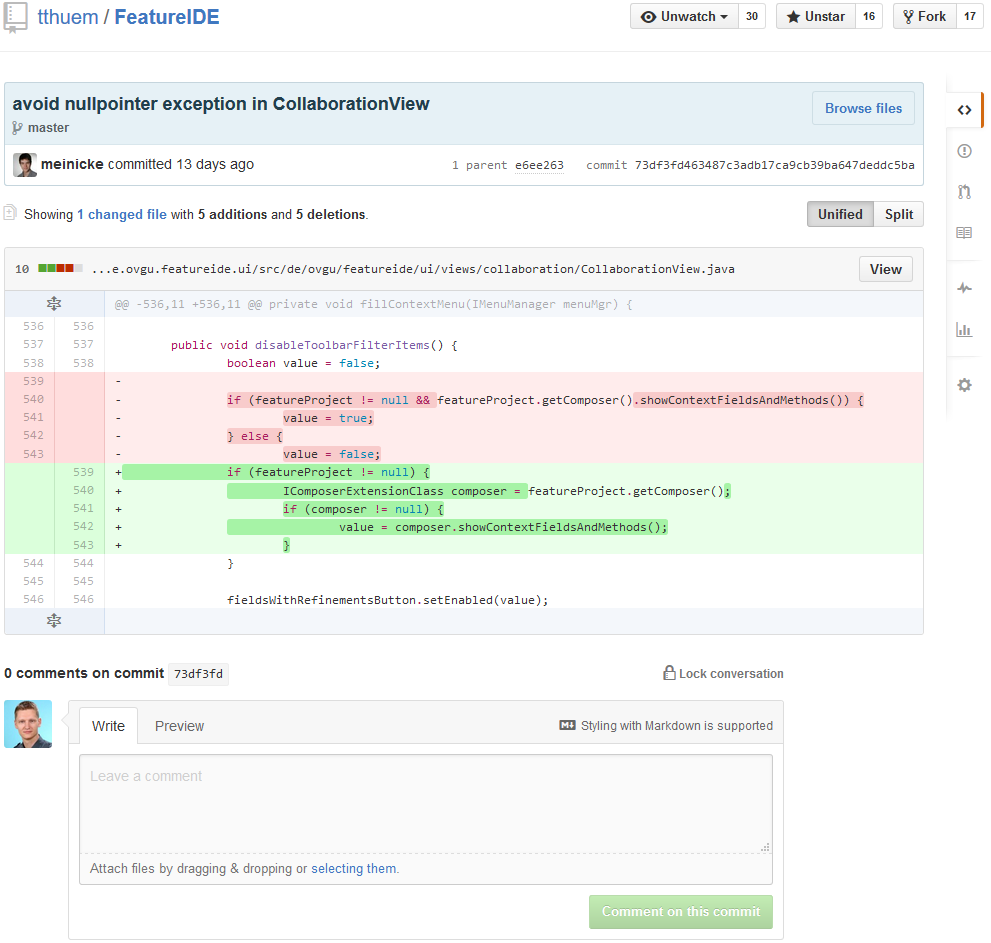
\includegraphics[height=.9\textheight]{../pics/codereview/github2}}
\end{frame}

\lessonslearned{
	\item What is quality, quality assurance, product quality, quality in use?
	\item Terms: software testing, validation / defect testing, validation / verification, development / release / user testing, manual / automated testing, constructive / analytical / organizational quality assurance
	\item Code reviews
	\item Next: How to cover all parts of a program?
}{
	\item \sommerville, Chapter 8 Software Testing
	\item \ludewiglichter, Chapter 5 \deutsch{Software-Qualität} and Chapter 13 \deutsch{Software-Qualitätssicherung und -Prüfung}
}{
	\begin{enumerate}
		\item<+-> Form in groups of 2--3 students
		\item<+-> Discuss own examples for insufficient product quality
		\item<+-> Can you assign the right kind of product quality for each example?\\~\\functional suitability, security, reliability, usability, compatibility, performance efficiency, maintainability, portability (see Slide~\ref{slide:productquality})
			\lectureqr{03}
	\end{enumerate}
}
	%	\item Open your favorite IDE and write a small example program illustrating one error detected by the Java compiler
	%	\item Upload a screenshot of your program in Moodle including a brief description of the error: \url{https://moodle.uni-ulm.de/mod/moodleoverflow/discussion.php?d=2127}
	%	\item Do a code review for another example (i.e., comment on possible improvements)
	%	\item See \href{https://moodle.uni-ulm.de/mod/moodleoverflow/discussion.php?d=3866}{Moodle} % TODO in 2023 update link
	%	\item Think of a change to the modulo method (cf.\ previous slide) that would be classified as error or warning by the Java compiler
	%	\item Do a code review of the \href{https://github.com/tthuem/2020WS-SWT-Calculator/blob/testinglecturev0/ModuloExample/src/de/uulm/sp/swt/moduloexample/ModuloExample.java}{modulo method} (i.e., comment on possible improvements) % TODO in 2023 update link
	%	\item Submit your results in Moodle and inspect other submissions
	%\item[] Answer the quiz in Moodle to track your learning progress of this chapter
	%\\\hfill\fancyqr{https://moodle.uni-ulm.de/course/view.php?id=42562\#section-7}

\slideonly{
	\addtocounter{framenumber}{-1}
	\againframe<7>{productquality}
}

\section{White-Box Testing}
\begin{frame}
	\begin{fancycolumns}[height=8.5cm]
		\pic[width=\linewidth,trim=0 425 0 75,clip]{people/edsger-dijkstra}
		\vspace{-7mm}
		
		\begin{note}{Edsger W. Dijkstra (1972) \mysource{\thehumbleprogrammer}}
			\mycite{Program testing can be a very effective way to show the presence of bugs, but it is hopelessly inadequate for showing their absence.}
		\end{note}
		% 1930-2002, ACM Turing Award winner
		\nextcolumn
		%\href{}{\includegraphics[width=\linewidth,trim=0 0 0 0,clip]{burt-rutan}}
		\vspace{56mm}
		
		\begin{note}{Burt Rutan \mysource{\href{https://www.routledge.com/Design-of-Biomedical-Devices-and-Systems-4th-edition/King-Fries-Johnson/p/book/9781138723061}{King~et~al.\ 2018}}}
			\mycite{Testing leads to failure, and failure leads to understanding.}
		\end{note}
		% unclear
	\end{fancycolumns}
\end{frame}

\subsection{Test Cases}
\begin{frame}{\insertsubsection\ \deutschertitel{Testfälle}}
	\begin{fancycolumns}[animation=none]
		\uncover<1->{
			\begin{definition}{Systematic Test \mysource{\ludewiglichter}}
				A systematic test is a test, in which
				\begin{itemize}
					\item[1.] the setup is defined,
					\item[2.] the inputs are chosen systematically,
					\item[3.] the results are documented and evaluated by criteria being defined prior to the test. 
				\end{itemize}
			\end{definition}
		}
		\uncover<2->{
			\begin{definition}{Test Case \mysource{\ludewiglichter}}
				In a test, a number of test cases are executed, whereas each test case consists \emph{input values} for a single execution and \emph{expected outputs}. An \emph{exhaustive test} refers a test in which the test cases exercise all the possible inputs.
			\end{definition}
		}
		\nextcolumn
		\uncover<3->{
			\begin{example}{Exhaustive Testing in Practice?}
				\texttt{boolean a, b, c;}\\			
				\texttt{int i, j;}\\~\\
				\texttt{bla(a,b,c)} \uncover<4->{has $2^3 = 8$ possible inputs}\\
				\texttt{blub(i,j)} \uncover<5->{has $(2^{32})^2 = 2^{64} \approx 10^{19}$ inputs}
				\uncover<6->{\begin{itemize}
						\item assuming $10^9$ test cases can be executed in 1~second (cf.\ CPU with more than 1 GHz)
						\item exhaustive test of \texttt{blub} takes $\approx 585$ years
						\item testing for a day would cover less than 0.0005 \% of the inputs
				\end{itemize}}
				\uncover<7->{How to test thousands of such methods several times a day?}
			\end{example}
		}
	\end{fancycolumns}
\end{frame}

\subsection{Test-Case Design}
\begin{frame}{\insertsubsection\ \deutschertitel{Testfallentwurf}}
	\begin{fancycolumns}
		\begin{note}{Goal \mysource{\ludewiglichter}}
			Detect a large number of failures with a low number of test cases. A test case (execution) is \emph{positive}, if it detects a failure, and \emph{successful} if it detects an unknown failure.
		\end{note}
		\begin{definition}{An ideal test case is \ldots \mysource{\ludewiglichter}}
			\begin{itemize}
				\item representative: represents a large number of feasible test cases
				\item failure sensitive: has a high probability to detect a failure
				\item non-redundant: does not check what other test cases already check
			\end{itemize}
		\end{definition}
		\nextcolumn
		\\\vspace{-7mm}
		\hfill
		\begin{tikzpicture}
			\path[small mindmap,
			every node/.style={concept,font=\scriptsize},
			emph/.style={font=\bfseries\scriptsize},
			concept color=foreground!20!background]
			node {Test-Case Design}
			child[concept color=blue!20!background,visible on={<2->}] { node {experience-based} }
			child[concept color=green!20!background,visible on={<3->}] { node {structure-based} 
				child { node {white-box testing} }
			}
			child[concept color=orange!20!background,visible on={<4->}] { node {specification-based} 
				child { node {black-box testing} }
			}
			;
		\end{tikzpicture}
	\end{fancycolumns}
\end{frame}

\subsection{Modulo in Different Programming Languages}
\begin{frame}{\insertsubsection}
	\begin{fancycolumns}[widths={55}]
		\begin{exampletight}{Overview by Torsten Curdt:}
			\centering\picDark[height=60mm]{testing/modulo-negative}
		\end{exampletight}
		\nextcolumn
		\begin{exampletight}{An Own Modulo Implementation}
			\centering\pic[height=60mm]{testing/modulo-with-javadoc-small-nohint} % TODO in 2023 update link
		\end{exampletight}
	\end{fancycolumns}
\end{frame}

\tikzset{emph/.style={thick,draw=blue,fill=blue!10!background},e1/.style={},e2/.style={},e3/.style={},e4/.style={},e5/.style={},e6/.style={},e7/.style={},e8/.style={}}
\renewcommand{\cfg}{ % TODO hack as command already exists, rename consistently
	\begin{tikzpicture}[yscale=-.5,xscale=.866,every node/.style={draw,semithick,circle,fill=background},to/.style={->,>={Stealth[round]},semithick,}]
		\node[e1,e2,e3,e4,e5,e6,e7,e8] (1) at (0,0) {1};
		\node[e1,e4,e5] (2) at (1,1) {2};
		\node[e1,e2,e4,e5,e6,e7,e8] (3) at (0,2) {3};
		\node[e1,e2,e4,e5,e6,e7,e8] (4) at (0,4) {4};
		\node[e1,e5,e7,e8] (5) at (1,5) {5};
		\node[e1,e2,e8] (6) at (0,6) {6};
		\draw[to,e1,e4,e5] (1) to (2);
		\draw[to,e2,e6,e7,e8] (1) to (3);
		\draw[to,e1,e4,e5] (2) to (3);
		\draw[to,e1,e2,e4,e5,e6,e7,e8] (3) to (4);
		\draw[to,e1,e5,e7,e8] (4) to[bend right=20] (5);
		\draw[to,e1,e2,e8] (4) to (6);
		\draw[to,e1,e5,e7,e8] (5) to[bend right=20] (4);
	\end{tikzpicture}
}

\subsection{White-Box Testing}
\begin{frame}{\insertsubsection\ \deutschertitel{Strukturtest}}
	\begin{fancycolumns}[animation=none]
		\begin{definition}{White-Box Testing \mysource{\ludewiglichter}}
			\begin{itemize}
				\setlength\itemsep{.1em}
				\item inner structure of test object is used
				\item idea: coverage of structural elements
				\item code translated into control flow graph
				\item specific test case (concrete inputs)\\derived from logical test case (conditions)\\derived from path in control flow graph
			\end{itemize}
		\end{definition}
		\uncover<2->{
			\begin{exampletight}{}
				\pic[width=\linewidth]{testing/modulo}
			\end{exampletight}
		}
		\nextcolumn
		\\\vspace{33mm}
		{\only<4->{\tikzset{e2/.append style={emph}}}\only<3->{\cfg}}
		%\only<3->{\tikzset{e1/.append style={emph}}\cfg}
	\end{fancycolumns}
\end{frame}
% control flow graphs as activity diagrams: \umluserguide, Chapter~20, Modeling an Operation

\subsection{Coverage Criteria}
\begin{frame}{\insertsubsection\ \deutschertitel{Überdeckungskriterien}}
	\begin{fancycolumns}[animation=none]
		\begin{definition}{Coverage Criteria \mysource{\ludewiglichter}}
			\begin{itemize}
				\item[1.] statement coverage \deutsch{Anweisungsüberdeck.}: all statements are executed for at least one test case
				\uncover<3->{\item[2.] branching coverage \deutsch{Zweigüberdeckung}: statement coverage and for each branching statement all branches have been exercised} % TODO not so easy to define as percentage
				\uncover<4->{\item[3.] term coverage \deutsch{Termüberdeckung}: branching coverage and terms ($n$) used in a branching statement are combined exhaustively ($2^n$)\hfill(simplified)}
				% TODO discuss path coverage?
			\end{itemize}
		\end{definition}
		\vspace{-1mm}
		\uncover<2->{\small
			\begin{example}{In Practice}
				100\% statement coverage not feasible in presence of dead code or some unreachable error handling
				
				\uncover<5->{100\% term coverage not feasible for certain dependencies between choices: \texttt{even() || odd()}}
			\end{example}
		}
		\nextcolumn
	\end{fancycolumns}
\end{frame}

\subsection{Statement Coverage}
\begin{frame}
	\begin{fancycolumns}[t,animation=none]
		\begin{exampletight}{Statement Coverage for Modulo Example}
			\pic[width=\linewidth]{testing/modulo}
		\end{exampletight}
		\begin{example}{First Test Case}
			\setlength\tabcolsep{.5mm}
			\begin{tabularx}{\textwidth}{rl}				
				path: & \uncover<2->{1}\uncover<3->{, 2, 3, 4}\uncover<4->{, 5, 4}\uncover<5->{, 6}\\
				logical test case: & \uncover<3->{$b < 0$}\uncover<4->{ $\wedge$ $a > -b$}\uncover<5->{ $\wedge$ $a+b \leq -b$}\\
				specific test case: & \uncover<6->{$a = 5$, $b = -3$}\\
				expected result: & \uncover<7->{$m = 2$}
			\end{tabularx}
		\end{example}
		\nextcolumn
		\\[5mm]
		\only<1|handout:0>{\cfg}%
		\only<2|handout:0>{\tikzset{e3/.append style={emph}}\cfg}%
		\only<3|handout:0>{\tikzset{e4/.append style={emph}}\cfg}%
		\only<4|handout:0>{\tikzset{e5/.append style={emph}}\cfg}%
		\only<5->{\tikzset{e1/.append style={emph}}\cfg}%
		\uncover<8->{\correct}
	\end{fancycolumns}
\end{frame}

\subsection{Branching Coverage}
\begin{frame}[plain]
	\begin{fancycolumns}[t,animation=none]
		\begin{exampletight}{Branching Coverage for Modulo Example}
			\pic[width=\linewidth]{testing/modulo}
		\end{exampletight}
		\vspace{-1mm}
		\begin{example}{First Test Case}
			\setlength\tabcolsep{.5mm}
			\begin{tabularx}{\textwidth}{rl}				
				path: & 1, 2, 3, 4, 5, 4, 6\\
				logical test case: & $b < 0$ $\wedge$ $a > -b$ $\wedge$ $a+b \leq -b$\\
				specific test case: & $a = 5$, $b = -3$ and $m = 2$
			\end{tabularx}
		\end{example}
		\vspace{-1mm}
		\begin{example}{Second Test Case}
			\setlength\tabcolsep{.5mm}
			\begin{tabularx}{\textwidth}{rl}				
				path: & \uncover<2->{1}\uncover<3->{, 3, 4}\uncover<4->{, 6}\\
				logical test case: & \uncover<3->{$b \geq 0$}\uncover<4->{ $\wedge$ $0 \leq a \leq b$}\\
				specific test case: & \uncover<5->{$a = 0$, $b = 5$}\uncover<6->{ and $m = 0$}
			\end{tabularx}
		\end{example}
		\nextcolumn
		\\[5mm]
		{\tikzset{e1/.append style={emph}}\cfg}
		\only<1|handout:0>{\cfg}%
		\only<2|handout:0>{\tikzset{e3/.append style={emph}}\cfg}%
		\only<3|handout:0>{\tikzset{e6/.append style={emph}}\cfg}%
		\only<4->{\tikzset{e2/.append style={emph}}\cfg}%
		\uncover<7->{\correct}
		\\[15mm]
		\uncover<8->{\begin{note}{Ternary Operator in Statement 5}
				\begin{itemize}
					\item could also be treated as branching statement
					\item how to adapt the control flow graph then?
					\item are the two test cases still sufficient?
				\end{itemize}
		\end{note}}
	\end{fancycolumns}
\end{frame}

\subsection{Term Coverage}
\begin{frame}[plain]
	\begin{fancycolumns}[t,animation=none]
		\begin{exampletight}{Term Coverage for Modulo Example}
			\pic[width=\linewidth]{testing/modulo}
		\end{exampletight}
		\vspace{-1mm}
		\begin{example}{}
			\setlength\tabcolsep{.5mm}
			\begin{tabularx}{\textwidth}{rl}				
				logical test case: & $b < 0$ $\wedge$ $a > -b$ $\wedge$ $a+b \leq -b$\\
				specific test case: & $a = 5$, $b = -3$ and $m = 2$\uncover<14->{\correct}
			\end{tabularx}
		\end{example}
		\vspace{-1mm}
		\begin{example}{}
			\setlength\tabcolsep{.5mm}
			\begin{tabularx}{\textwidth}{rl}				
				logical test case: & $b \geq 0$ $\wedge$ $0 \leq a \leq b$\\
				specific test case: & $a = 0$, $b = 5$ and $m = 0$\uncover<14->{\correct}
			\end{tabularx}
		\end{example}
		\vspace{-1mm}
		\begin{example}{}
			\setlength\tabcolsep{.5mm}
			\begin{tabularx}{\textwidth}{rl}				
				path: & \uncover<8->{1}\uncover<9->{, 3, 4}\uncover<10->{, 5, 4}\uncover<11->{, 6}\\
				logical test case: & \uncover<9->{$b \geq 0$}\uncover<10->{ $\wedge$ $a < 0$}\uncover<11->{ $\wedge$ $0 \leq a+b \leq b$}\\
				specific test case: & \uncover<12->{$a = -2$, $b = 5$}\uncover<13->{ and $m = 3$}\uncover<14->{\correct}
			\end{tabularx}
		\end{example}
		\nextcolumn
		\\[5mm]
		{\tikzset{e1/.append style={emph}}\cfg}
		{\tikzset{e2/.append style={emph}}\cfg}
		\only<7|handout:0>{\cfg}%
		\only<8|handout:0>{\tikzset{e3/.append style={emph}}\cfg}%
		\only<9|handout:0>{\tikzset{e6/.append style={emph}}\cfg}%
		\only<10|handout:0>{\tikzset{e7/.append style={emph}}\cfg}%
		\only<11->{\tikzset{e8/.append style={emph}}\cfg}\\[5mm]
		\uncover<2->{$\neg(m < 0)$}\uncover<3->{ and $m > b$\correct}\\[5mm]
		\uncover<2->{$\neg(m < 0)$}\uncover<4->{ and $\neg(m > b)$\correct}\\[5mm]
		\uncover<5->{$m < 0$ and $m > b$}\uncover<6->{ impossible\only<15->{*}\alsocorrect}\\[5mm]
		\uncover<5->{$m < 0$ and $\neg(m > b)$}\uncover<13->{\correct}\\[3mm]
		\uncover<15->{\tiny*\,see third part of the lecture}
	\end{fancycolumns}
\end{frame}

\lessonslearned{
	\item Systematic test, exhaustive testing
	\item Test case: representative, failure sensitive, non-redundant
	\item Test-case design: experience-/structure-/specification-based
	\item Coverage in white-box testing: statement/branching/term coverage
	\item Next: How to cover all parts of the specification?
}{
	\item \ludewiglichter, Chapter 19 \deutsch{Programmtest}
}{
	\pic[width=\linewidth]{testing/modulo}
	\vspace*{-1ex}
	Determine the coverage of a test suite.
	\lectureqr{03}
}
	%	\item See \href{https://moodle.uni-ulm.de/mod/moodleoverflow/discussion.php?d=3867}{Moodle} % TODO in 2023 update link
	%	\item Watch screencast on how to do white-box testing with JUnit
	%	\item Implement a new operation in the calculator and update the white-box tests accordingly: \url{https://github.com/tthuem/2020WS-SWT-Calculator/tree/testinglecturev1} % TODO in 2023 update link
	%	\item Post your code changes and tests in Moodle
	%\item[] Determine the coverages of certain Modulo Test Cases in Moodle
	%\\\hfill\fancyqr{https://moodle.uni-ulm.de/course/view.php?id=42562\#section-7}

\section{Black-Box Testing}
\subsection{Black-Box Testing}
\begin{frame}{\insertsubsection\ \mytitlesource{\ludewiglichter}}
	\begin{fancycolumns}
		\begin{note}{Motivation}
			\begin{itemize}
				\item source code not always available (e.g., outsourced components, obfuscated code)
				\item specific test cases derived from logical ones using arbitrary values
				\item specification not incorporated so far (only for expected results)
				\item invalid inputs not tested
				\item errors are not equally distributed
			\end{itemize}
		\end{note}
		\begin{definition}{Black-Box Testing \deutsch{Funktionstest}}
			\begin{itemize}
				\item test-case design based on specification
				\item source code and its inner structure is ignored (assumed as a black-box)
			\end{itemize}
		\end{definition}
		\nextcolumn
		\vspace{-5mm}
		\begin{definition}{1. Equivalence Class Testing}
			\begin{itemize}
				\item idea: classify inputs and outputs into equivalence classes
				\item assumption: equivalent test cases detect the same faults, one test case is sufficient
			\end{itemize}
		\end{definition}
		\begin{definition}{2. Boundary Testing}
			\begin{itemize}
				\item extension of equivalence class testing
				\item goal: use experience (e.g., off-by-one errors)
				\item for every equivalence class: consider smallest, typical, and largest value
			\end{itemize}
		\end{definition}
		\begin{example}{In Practice}
			\begin{itemize}
				\item often combinations of white-box and black-box testing
				\item more techniques with requirements or design
			\end{itemize}
		\end{example}
	\end{fancycolumns}
\end{frame}

\subsection{Equivalence Class Testing}
\begin{frame}{\insertsubsection}
	\begin{fancycolumns}[columns=3,widths={46,4,50},animation=none]
		\begin{exampletight}{JavaDoc Specification for Modulo Example}
			\pic[width=\linewidth]{testing/modulo-only-javadoc-small-nohint}
		\end{exampletight}
		\begin{example}{Equivalence Classes}
			\begin{itemize}
				\item input a: $a < 0$, $a \geq 0$
				\item input b: $b < 0$, $b \geq 0$
				\item output: $m = 0$, $m > 0$, exception
			\end{itemize}
		\end{example}
		\nextcolumn
		\nextcolumn
		\uncover<2->{
			\begin{example}{Test Cases}
				\begin{tabular}{c c c c}	% temp
					% TODO: fix M{c}{num-}
					%\begin{tabular}{M{c}{1-} M{c}{4-} M{c}{5-} M{c}{6-}}
					& TC1 & TC2 & TC3 \\
					\toprule
					$a < 0$ & X &  &  \\
					$a \geq 0$ &  & X & X \\
					\midrule
					$b < 0$ & X &  &  \\
					$b > 0$ &  & X &  \\
					$b = 0$ &  &  & X \\
					\midrule
					$m = 0$ & X &  &  \\
					$m > 0$ &  & X &  \\
					exception &  &  & X \\
					\midrule
					\uncover<3->{input a & -3 & 1 & 2} \\
					\uncover<3->{input b & -3 & 2 & 0} \\
					\uncover<3->{expected output & 0 & 1 & exception} \\
					\midrule
					\uncover<4->{result & 0\correct & 1\correct & timeout\wrong} \\
					\bottomrule
				\end{tabular}
			\end{example}
		}
	\end{fancycolumns}
\end{frame}

\subsection{Boundary Testing}
\begin{frame}{\insertsubsection}
	\begin{fancycolumns}[columns=3,widths={4,92}]
		\nextcolumn
		\begin{example}{Test Cases}
			\begin{tabular}{c c c c c c c c}	% temp
				% TODO: fix M{c}{num-}
				%\begin{tabular}{M{c}{1-} M{c}{1-} M{c}{1-} M{c}{1-} M{c}{2-} M{c}{3-} M{c}{4-} M{c}{5-}}
				& TC1 & TC2 & TC3 & TC4 & TC5 & TC6 & TC7 \\
				\toprule
				$a < 0$ & X &  &  & min & max &  &  \\
				$a \geq 0$ &  & X & X &  &  & min & max \\
				\midrule
				$b < 0$ & X &  &  & max &  & min &  \\
				$b > 0$ &  & X &  &  & max &  & min \\
				$b = 0$ &  &  & X &  &  &  &  \\
				\midrule
				$m = 0$ & X &  &  & X &  & X & X \\
				$m > 0$ &  & min &  &  & max &  &  \\
				exception &  &  & X &  &  &  &  \\
				\midrule
				\uncover<1->{input a & -3 & 1 & 2 & minInt & -1 & 0 & maxInt }\\
				\uncover<1->{input b & -3 & 2 & 0 & -1 & maxInt & minInt & 1 }\\
				\uncover<1->{expected output & 0 & 1 & exception & 0 & maxInt-1 & 0 & 0 }\\
				\midrule
				\uncover<2->{result & 0\correct & 1\correct & timeout\wrong & 0\correct & maxInt-1\correct & timeout\wrong & 1\wrong }\\
				\bottomrule
			\end{tabular}
		\end{example}
		\nextcolumn
	\end{fancycolumns}
\end{frame}
%// a smallest negative, b largest negative, smallest result
%assertEquals(0,ModuloExample.modulo(Integer.MIN_VALUE,-1));
%// a largest negative, b largest positive, largest result
%assertEquals(Integer.MAX_VALUE-1,ModuloExample.modulo(-1,Integer.MAX_VALUE));
%// a smallest positive, b smallest negative, smallest result
%//assertEquals(0,ModuloExample.modulo(0,Integer.MIN_VALUE)); // leads to endless loop for every a
%assertEquals(0,ModuloExample.modulo(0,Integer.MIN_VALUE+1));
%// a largest positive, b smallest positive, smallest result
%assertEquals(0,ModuloExample.modulo(Integer.MAX_VALUE,1));

\subsection{Detected Faults in Modulo Example}
\begin{frame}
	\begin{fancycolumns}[animation=none]
		\uncover<1->{
			\begin{exampletight}{Detected Faults in Modulo Example}
				\pic[width=\linewidth]{testing/modulo}
			\end{exampletight}
			\vspace{-1mm}
			\begin{example}{}
				\wrong~~~~TC3: infinite loop for $b = 0$,\\ missing exception compared to JavaDoc
			\end{example}
		}
		\vspace{-1mm}
		\uncover<2->{
			\begin{example}{}
				\wrong~~~~TC6: $b$ remains negative as\\ \texttt{-Integer.MIN\_VALUE == Integer.MIN\_VALUE}\\ and the loop condition is fulfilled for any integer
			\end{example}
		}
		\vspace{-1mm}
		\uncover<3->{
			\begin{example}{}
				\wrong~~~~TC7: indicates that $m > b$ in the loop condition should be fixed to $m \geq b$
			\end{example}
		}
		\nextcolumn
		\uncover<4->{
			\begin{exampletight}{Improved Modulo Example}
				\pic[width=\linewidth]{testing/modulo-fixed}
			\end{exampletight}
		}
		\vspace{-1mm}
		\uncover<5->{
			\begin{example}{Passes All Test Cases}
				\vspace{3mm}
				\correct~~~~~\correct~~~~~\correct~~~~~\correct~~~~~\correct~~~~~\correct~~~~~\correct~~~~~\correct~~~~~\correct~~~~~\correct~~~~~ 
			\end{example}
		}
	\end{fancycolumns}
\end{frame}

\subsection{Reasons for Positive Test Cases}
\begin{frame}{\insertsubsection}
	\begin{fancycolumns}
		\begin{note}{Reasons for Positive Test Cases}
			\begin{itemize}
				\item actual fault
				\uncover<2->{\item wrong test case (input and expected results do not match)}
				\uncover<3->{\item interaction with other programs/libraries
					\item fault in the compiler
					\item fault in the operating system / device drivers
					\item fault in the hardware or hardware defect
					\item not enough memory
					\item does not halt (cf.\ undecidability of the halting problem)
					\item bitflip due to cosmic ray
					\item \ldots}
			\end{itemize}
		\end{note}
		%		\mynote{Reasons for Negative Test Cases}{
			%			\begin{itemize}
				%				\setlength\itemsep{.5em}
				%				\item program correct
				%				\item see above
				%			\end{itemize}
			%		}
	\end{fancycolumns}
\end{frame}

\begin{frame}
	\begin{fancycolumns}[height=8.5cm]
		\pic[width=\linewidth,trim=0 425 0 75,clip]{people/edsger-dijkstra}
		\vspace{-7mm}
		
		\begin{note}{Edsger W. Dijkstra \mysource{\goodliffe}}
			\mycite{If debugging is the process of removing software bugs, then programming must be the process of putting them in.}
		\end{note}
		% 1930-2002, ACM Turing Award winner
		\nextcolumn
		\pic[width=\linewidth,trim=250 0 0 0,clip]{people/brian-kernighan}
		\vspace{-7mm}
		
		\begin{note}{Brian Kernighan (1978) \mysource{\elementsofprogrammingstyle}}
			\mycite{Everyone knows that debugging is twice as hard as writing a program in the first place. So if you're as clever as you can be when you write it, how will you ever debug it?}
		\end{note}
		% known for books on C and Go
	\end{fancycolumns}
\end{frame}

\lessonslearned{
	\item Black-box testing: equivalence class testing and boundary testing
	\item Even systematic testing cannot ensure finding all faults
	\item Next: Never change a running system! How realistic is that?
}{
	\item \ludewiglichter, Chapter 19 \deutsch{Programmtest}
}{
	Quiz in Stud.IP
	\lectureqr{03}
}
	%	\item See \href{https://moodle.uni-ulm.de/mod/moodleoverflow/discussion.php?d=3868}{Moodle} % TODO in 2023 update link
	%	\item Watch screencast on how to do black-box testing with JUnit
	%	\item Extend the black-box tests of the calculator for your new operation: \url{https://github.com/tthuem/2020WS-SWT-Calculator/tree/testinglecturev2}
	%	\item Post your changed code and tests in Moodle
	%	\item[] Live Coding Exercise for JUnit, see Moodle for instructions and solutions
	%\\\hfill\fancyqr{https://moodle.uni-ulm.de/course/view.php?id=42562\#section-7}
%	\item[] Answer the quiz in \panda{} to track your learning progress of this chapter
%	\\\hfill\fancyqr{https://panda.uni-paderborn.de/mod/quiz/view.php?id=2744505} 

%\faq{
%	\item
%}{
%	\item
%}{
%	\item
%}

% TODO L04 SOFTWARE CHANGES

\ifuniversity{tubs}{\date{November 5, 2024}}

\author{Thomas Thüm}
\lecture{Software Changes}{changes}

\begin{frame}{\insertsubtitle}
	\alt<3->{
		\projectcartoon{01}{how the customer explained it}
		\projectcartoon{02}{how the project leader understood it}
		\projectcartoon{03}{how the analyst designed it}
		\projectcartoon{04}{how the programmer implemented it}
	}{
		\hprojectcartoon{01}{how the customer explained it}
		\hprojectcartoon{02}{how the project leader understood it}
		\hprojectcartoon{03}{how the analyst designed it}
		\hprojectcartoon{04}{how the programmer implemented it}
	}%
	\uncover<2->{\hprojectcartoon{18}{how patches were applied\\~\\\textbf{software\\changes}}}
\end{frame}

\section{Software Maintenance}
\subsection{Software Maintenance in Practice}

\subsubsection{New Year's Eve for Maintainers}
\begin{frame}{New Year's Eve: Party Time?!?}
	\begin{fancycolumns}
		\pic[width=\linewidth,trim=0 230 0 140,clip]{changes/london-fireworks}
		\vspace{-7mm}
		
		\begin{example}{}
			London Eye on January 1st, \sout{2008} 2017
		\end{example}
	\end{fancycolumns}
\end{frame}

\begin{frame}{\insertsubsubsection}
	\begin{fancycolumns}
		\begin{exampletight}{Meanwhile in the Internet}
			\picDark[width=\linewidth,trim=0 0 0 0,clip]{changes/cloudflare-offline}
		\end{exampletight}
		\nextcolumn
		\picDark[width=\linewidth,trim=0 0 0 0,clip]{changes/cloudflare-dns-control-panel}
		\vspace{-7mm}
		
		\begin{example}{Meanwhile in San Francisco \mysource{\href{https://blog.cloudflare.com/how-and-why-the-leap-second-affected-cloudflare-dns/}{cloudflare.com}}}
			\mycite{\emph{At midnight UTC} on New Year’s Day, deep inside Cloudflare’s custom RRDNS software, a number went negative when it should always have been, at worst, zero. [\ldots] %A little later this negative value caused RRDNS to panic. This panic was caught using the recover feature of the Go language. The net effect was that some DNS resolutions to some Cloudflare managed web properties failed.
				%The problem only affected customers who use CNAME DNS records with Cloudflare, and only affected a small number of machines across Cloudflare's 102 data centers.
				At peak approximately \emph{0.2\% of DNS queries} to Cloudflare were affected and less than \emph{1\% of all HTTP requests to Cloudflare encountered an error}.}
		\end{example}
	\end{fancycolumns}
\end{frame}

\subsubsection{Maintenance at Work}
\begin{frame}{\insertsubsubsection\ \mytitlesource{\href{https://blog.cloudflare.com/how-and-why-the-leap-second-affected-cloudflare-dns/}{cloudflare.com}}}
	\begin{fancycolumns}
		\begin{example}{Meanwhile in San Francisco}
			\mycite{This problem was quickly identified. The most affected machines were \emph{patched in 90 minutes} and the fix was \emph{rolled out worldwide by 06:45 UTC}. We are sorry that our customers were affected, but we thought it was worth writing up the root cause for others to understand.}
		\end{example}
		
		\begin{exampletight}{The Timeline}
			\picDark[width=\linewidth,trim=0 0 0 0,clip]{changes/cloudflare-timeline}
		\end{exampletight}
		\nextcolumn
		\begin{exampletight}{Monitoring}
			\picDark[width=\linewidth,trim=0 0 0 0,clip]{changes/cloudflare-timeline-diagram}
		\end{exampletight}
		
		\begin{note}{Fun Fact}
			San Francisco's standard time zone is UTC-8
		\end{note}
	\end{fancycolumns}
\end{frame}

%\subsection{Wisdom on Debugging}
%\begin{frame}{\insertsubsection}
%	\begin{fancycolumns}
%		\pic[width=\linewidth,trim=35 0 0 0,clip]{people/gordon-glegg}
%		\vspace{-7mm}
%		
%		\begin{note}{Gordon Glegg \mysource{\href{https://twitter.com/CodeWisdom/status/1140295217947512833}{twitter.com}}}
%			\mycite{Sometimes the problem is to discover what the problem is.}
%		\end{note}
%		\nextcolumn
%		\pic[width=\linewidth,trim=0 80 0 25,clip]{people/jessica-joy-kerr}
%		\vspace{-7mm}
%		
%		\begin{note}{Jessica Joy Kerr (2020) \mysource{\href{https://jessitron.com/2020/02/07/smaller-pieces-lower-pain/}{jessitron.com}}}
%			\mycite{In programming, it’s dangerous to work near your working memory threshold. You get more mistakes and more complicated code.}
%		\end{note}
%	\end{fancycolumns}
%\end{frame}

\subsubsection{The One-Character-Fix}
\begin{frame}{\insertsubsubsection\ \mytitlesource{\href{https://blog.cloudflare.com/how-and-why-the-leap-second-affected-cloudflare-dns/}{cloudflare.com}}}
	\begin{fancycolumns}
		\begin{exampletight}{The Patch}
			\picDark[width=\linewidth,trim=0 0 0 0,clip]{changes/cloudflare-fix}
		\end{exampletight}
		\nextcolumn
		\begin{example}{A Falsehood Programmers Believe About Time}
			\mycite{The root cause of the bug that affected our DNS service was the belief that \emph{time cannot go backwards}. In our case, some code assumed that the difference between two times would always be, at worst, zero.
				
				~
				
				RRDNS is written in Go and uses Go’s time.Now() function to get the time. Unfortunately, this function does not guarantee monotonicity.}
		\end{example}
	\end{fancycolumns}
\end{frame}

\subsubsection{Leap Seconds}
\begin{frame}{\insertsubsubsection\ \deutsch{Schaltsekunden}}
	\begin{fancycolumns}
		\centering\pic[width=.7\linewidth,trim=0 0 0 0,clip]{changes/leap-second}
		
		\begin{exampletight}{Leap Second 37 \mysource{\href{https://www.spinellis.gr/blog/20170101/}{spinellis.gr}}}
			\picDark[width=\linewidth,trim=0 0 0 0,clip]{changes/leap-second-37}
		\end{exampletight}
		\nextcolumn
		\begin{exampletight}{27 Leap Seconds since 1972 \mysource{\href{https://en.wikipedia.org/wiki/Leap_second}{wikipedia.org}}}
			\hfill\picDark[width=.25\linewidth,trim=0 0 0 0,clip]{changes/leap-seconds1}
			\hfill\picDark[width=.25\linewidth,trim=0 0 0 0,clip]{changes/leap-seconds2}
			\hfill\picDark[width=.25\linewidth,trim=0 0 0 0,clip]{changes/leap-seconds3}
			\hfill{}
		\end{exampletight} % 190% screenshots with 20 lines
	\end{fancycolumns}
\end{frame}

\xkcdframe{2266} % leap second/day smearing

\subsection{Software Maintenance}
\begin{frame}{\insertsubsection\ \mytitlesource{\ludewiglichter}}
	\begin{fancycolumns}
		\begin{note}{Motivation}
			\begin{itemize}
				\item for software: no compensation of deterioration, repair, spare parts
				\item corrections (especially shortly after first delivery)
				\item modification and reconstruction
			\end{itemize}
		\end{note}
		\nextcolumn
		\begin{definition}{Operation and Maintenance Phase \mysource{\ieeesixten}}
			\mycite{The period of time in the software life cycle during which a software product is employed in its operational environment, monitored for satisfactory performance, and modified as necessary to correct problems or to respond to changing requirements.}
		\end{definition}
		\begin{definition}{Maintenance \mysource{\ieeesixten}}
			\mycite{The process of modifying a software system or component after delivery to correct faults, improve performance or other attributes, or adapt to a changed environment.}
		\end{definition}
	\end{fancycolumns}
\end{frame}
% TODO Operations

\subsection{Kinds of Maintenance}
\begin{frame}{\insertsubsection\ \mytitlesource{\ludewiglichter}}
	\begin{fancycolumns}
		\begin{definition}{Adaptive Maintenance \mysource{\lientzswanson}}
			\mycite{Software maintenance performed to make a computer program usable in a changed environment.} \hfill \deutsch{adaptive Wartung}
		\end{definition}
		\begin{example}{}
			desktop application for a new version of an operating system (e.g., from Windows 8.1 to 10)
		\end{example}
		\begin{definition}{Corrective Maintenance \mysource{\lientzswanson}}
			\mycite{Maintenance performed to correct faults in software.} \hfill \deutsch{korrektive Wartung}
		\end{definition}
		\begin{example}{}
			Windows calculator showing wrong formulas
		\end{example}
		\nextcolumn
		% TODO it is really annoying that this category has an overlap with preventive maintenance, as better maintainability typically also results in fewer problems
		\begin{definition}{Perfective Maintenance \mysource{\lientzswanson}}
			\mycite{Software maintenance performed to improve the performance, maintainability, or other attributes of a computer program.} \hfill \deutsch{perfektive Wartung}
		\end{definition}
		\begin{example}{}
			better handling of very large files in a text editor
		\end{example}
		\begin{definition}{Preventive Maintenance \mysource{\lientzswanson}}
			\mycite{Maintenance performed for the purpose of preventing problems before they occur.} \hfill \deutsch{präventive Wartung}
		\end{definition}
		\begin{example}{}
			2,000 year problem, leap seconds/years
		\end{example}
	\end{fancycolumns}
\end{frame}
% TODO add links to original literature

\subsection{Wisdom on Maintenance}
\begin{frame}{\insertsubsection}
	\begin{fancycolumns}
		\pic[width=\linewidth,trim=0 360 0 50,clip]{people/karolina-szczur}
		\vspace{-7mm}
		
		\begin{note}{Karolina Szczur \mysource{\href{https://twitter.com/codewisdom/status/1141686386103332864}{twitter.com}}}
			\mycite{Writing software as if we are the only person that ever has to comprehend it is one of the biggest mistakes and false assumptions that can be made.}
		\end{note}
		\nextcolumn
		\pic[width=\linewidth,trim=450 235 450 120,clip]{changes/psychopath}
		\vspace{-7mm}
		
		\begin{note}{John F. Woods \mysource{\href{https://groups.google.com/g/comp.lang.c++/c/rYCO5yn4lXw/m/oITtSkZOtoUJ}{google.com}}}
			\mycite{Always code as if the guy who ends up maintaining your code will be a violent psychopath who knows where you live.}
		\end{note}
	\end{fancycolumns}
\end{frame}


\lessonslearned{
	\item Maintenance problems caused by leap seconds
	%\item Solutions: consider negative intervals, leap second smearing
	%\item Time pressure for maintenance
	%\item Develop software for maintenance
	\item Maintenance (Phase)
	\item Kinds of maintenance: adaptive, corrective, perfective, preventive
	%\item Reengineering = reverse engineering + restructuring + forward engineering
	\item Next: How to develop software that can be maintained?
}{
	\item \ludewiglichter, Chapter 22 \deutsch{Software-Wartung} %and 23 \\deutsch{Reengineering}
}{
	\begin{enumerate}
		\item<+-> Form groups of 2-3 students for Think-Pair
		\item Think (2 min): choose a kind of maintenace (e.g., preventive) and think of an example
		\item Pair (5 min): explain example to your group and let collegues guess whether it is adaptive, corrective, perfective or preventive maintenance
		%\item<+-> Which software maintenance has affected you? How long did it take to fix it?
		%\item<+-> Discuss your examples with your colleagues
	\end{enumerate}
}

% TODO skipped lecture part to make room for black-box testing
%\section{}
%%\input{content/}
%\lessonslearned{
%	\item Next: ...
%}{
%	\item ...
%}{
%	\begin{enumerate}
%		\item<+-> Form groups of 2-3 students
%	\end{enumerate}
%}

\section{Software Evolution}
\subsection{Evolution and Maintenance}
\begin{frame}{\insertsubsection\ \mytitlesource{\ludewiglichter}}
	\slideEvolutionAndMaintenance
\end{frame}

\subsection{Avoiding Complexity}
\begin{frame}{\insertsubsection}
	\begin{fancycolumns}
		\pic[width=\linewidth,trim=10 0 10 0,clip]{people/richard-pattis}
		\vspace{-7mm}
		
		\begin{note}{Richard E.\ Pattis \mysource{\href{https://www.cs.cmu.edu/~pattis/quotations.html}{cmu.edu}}}
			\mycite{When debugging, novices insert corrective code; experts remove defective code.}
		\end{note}
		% American professor, author of the educational programming language Karel
		\nextcolumn
		\pic[width=\linewidth,trim=0 120 0 30,clip]{people/ken-thompson}
		\vspace{-7mm}
		
		\begin{note}{Ken Thompson (born 1943) \mysource{\href{https://twitter.com/CodeWisdom/status/1386049811800109056}{twitter.com}}}
			\mycite{One of my most productive days was throwing away 1,000 lines of code.}
		\end{note}
		% Turing Award 1983, inventor of the programming language B (predecessor of C) and Go, UTF-8 encoding
	\end{fancycolumns}
\end{frame}

\widexkcdframe{1667} % complexity comes with changes over time

\subsection{Increasing Complexity}
\begin{frame}{\insertsubsection}
	\begin{fancycolumns}
		\pic[width=\linewidth,trim=0 200 0 600,clip]{people/tony-hoare}
		\vspace{-7mm}
		
		\begin{note}{Tony Hoare (born 1934) \mysource{\href{https://twitter.com/CodeWisdom/status/893532377586302977}{twitter.com}}}
			\mycite{Inside every large program, there is a small program trying to get out.}
		\end{note}
		% quicksort, hoare logic
		\nextcolumn
		\pic[width=\linewidth,trim=50 85 200 120,clip]{people/manny-lehman}
		\vspace{-7mm}
		
		\begin{note}{{Meir \mycite{Manny} Lehman (1925--2010) \mysource{\href{https://twitter.com/CodeWisdom/status/921139649661284352}{twitter.com}}}}
			\mycite{An evolving system increases its complexity unless work is done to reduce it.}
		\end{note}
		% known for laws on software evolution
	\end{fancycolumns}
\end{frame}

\subsection{Lehman's Laws of Software Evolution}
\begin{frame}{\insertsubsection\ \mytitlesource{\href{https://ieeexplore.ieee.org/iel3/5031/13795/00637156.pdf}{Lehman et al.\ 1997}}}
	\begin{fancycolumns}
		\begin{definition}{Lehman's Laws (excerpt)}
			\begin{itemize}
				\item Continuing Change: systems must be continually adapted to stay satisfactory % E-type systems must be continually adapted else they become progressively less satisfactorv.
				\item Increasing Complexity: complexity increases during evolution unless work is done to maintain or reduce it % As an E-type system evolves its complexity increases unless work is done to maintain or reduce it.
				%\item Self Regulation: %E-type system evolution process is self regulating with distribution of product and process measures close to normal.
				%\item Conservation of Organizational Stability (invariant work rate): %The average effective global activity rate in an evolving E-type system is invariant over product lifetime.
				\item Conservation of Familiarity: satisfactory evolution excludes excessive growth %As an E-type system evolves all associated with it, developers, sales personnel, users, for example, must maintain mastery of its content and behaviour to achieve satisfactory evolution. Excessive growth diminishes that mastery. Hence the average incremental growth remains invariant as the system evolves.
				\item Continuing Growth: functionality must be continually increased to maintain user satisfaction %The functional content of E-type systems must be continually increased to maintain user satisfaction over their lifetime.
				\item Declining Quality: quality will decline unless rigorously maintained and adapted to operational environment changes %The quality of E-type systems will appear to be declining unless they are rigorously maintained and adapted to operational environment changes.
				%\item Feedback System: %E-type evolution processes constitute multi-level, multi-loop, multi-agent feedback systems and must be treated as such to achieve significant improvement over any reasonable base.
			\end{itemize}
		\end{definition}
		\nextcolumn
		\begin{note}{Essence of the Laws}
			\begin{itemize}
				\item software that is used will be modified
				\item when modified, its complexity will increase (unless one does actively work against it)
			\end{itemize}
		\end{note}
		\begin{example}{Consequences}
			\begin{itemize}
				\item functional changes are inevitable
				\item changes are not necessarily a consequence of errors (e.g., in requirements engineering or programming)
				\item there are limits to what a development team can achieve (cf.\ Continuing Growth)
			\end{itemize}
		\end{example}
	\end{fancycolumns}
\end{frame}

\subsection{Simple and Clean}
\begin{frame}{\insertsubsection}
	\begin{fancycolumns}
		\pic[width=\linewidth,trim=0 35 0 40,clip]{people/grady-booch}
		\vspace{-7mm}
		
		\begin{note}{Grady Booch (born 1955) \mysource{\href{https://twitter.com/Grady_Booch/status/1035409406068813824}{twitter.com}}}
			\mycite{The function of good software is to make the complex appear to be simple.}
		\end{note}
		% known for UML
		\nextcolumn
		\pic[width=\linewidth,trim=800 700 800 600,clip]{people/robert-martin}
		\vspace{-7mm}
		
		\begin{note}{{Robert C.\ Martin (Uncle Bob, born 1952)}}
			Boy Scouts Rule: \mycite{Leave the campground cleaner than the way you found it.} \mysource{\href{https://learning.oreilly.com/library/view/97-things-every/9780596809515/ch08.html}{oreilly.com}}
		\end{note}
		% agile manifesto, book author
	\end{fancycolumns}
\end{frame}

\subsection{Code Refactoring}
\begin{frame}{\insertsubsection\ \mytitlesource{\sommerville}}
	\begin{fancycolumns}
		\begin{note}{Motivation}
			\begin{itemize}
				\item anticipating changes is typically infeasible
				\item anticipated changes may not materialize and unanticipated changes are required
				\item make changes easier by constantly refactoring the code
			\end{itemize}
		\end{note}
		\begin{definition}{Refactoring}
			\mycite{Refactoring means that the programming team looks for possible improvements to the software and implements them immediately. When team members see code that can be improved, they make these improvements even in situations where there is no immediate need for them.}
		\end{definition}
		\nextcolumn
		\begin{definition}{Structure of the Software}
			\mycite{A fundamental problem of incremental development is that local changes tend to \textbf{degrade the software structure}. Consequently, further changes to the software become harder and harder to implement. Essentially, the development proceeds by finding workarounds to problems, with the result that code is often duplicated, parts of the software are reused in inappropriate ways, and the overall structure degrades as code is added to the system. \textbf{Refactoring improves the software structure and readability and so avoids the structural deterioration that naturally occurs when software is changed.}}
		\end{definition}
	\end{fancycolumns}
\end{frame}

\subsection{Refactoring in Practice}
\begin{frame}{\insertsubsection}
	\begin{fancycolumns}
		\begin{example}{Theory vs Practice \mysource{\sommerville}}
			\mycite{In principle, when refactoring is part of the development process, the software should always be easy to understand and change as new requirements are proposed. In practice, this is not always the case. Sometimes \textbf{development pressure means that refactoring is delayed} because the time is devoted to the implementation of new functionality. Some new features and changes cannot readily be accommodated by code-level refactoring and \textbf{require that the architecture of the system be modified}.}
		\end{example}
		\nextcolumn
		\begin{note}{{Grandma Beck's Child-Rearing Philosophy}}
			\mycite{If it stinks, change it.} \mysource{\href{https://learning.oreilly.com/library/view/refactoring-improving-the/9780134757681/ch03.xhtml}{oreilly.com}}
		\end{note}
	\end{fancycolumns}
\end{frame}

\subsection{Smells and Refactorings} % TODO add examples for refactorings and smells
\begin{frame}{\insertsubsection\ \mytitlesource{\refactoring}}
	\begin{fancycolumns}
		\begin{definition}{Mysterious Name}
			\mycite{Puzzling over some text to understand what’s going on is a great thing if you’re reading a detective novel, but not when you’re reading code. [...] One of the most important parts of clear code is good names, so we put a lot of thought into naming functions, modules, variables, classes, so they clearly communicate what they do and how to use them.}\\--- Rename Method/Field/Variable Refactoring
		\end{definition}
		\nextcolumn
		\begin{definition}{Duplicated Code (aka.\ Code Clones)}
			\mycite{If you see the same code structure in more than one place, you can be sure that your program will be better if you find a way to unify them. Duplication means that every time you read these copies, you need to read them carefully to see if there’s any difference. If you need to change the duplicated code, you have to find and catch each duplication.}\\--- Extract/Pull-Up Method Refactoring
		\end{definition}
	\end{fancycolumns}
\end{frame}

\begin{frame}{\insertsubsection\ \mytitlesource{\refactoring}}
	\begin{fancycolumns}
		\begin{definition}{Long Method}
			\mycite{Since the early days of programming, people have realized that the longer a function is, the more difficult it is to understand. Older languages carried an overhead in subroutine calls, which deterred people from small functions. [...] [T]he real key to making it easy to understand small functions is good naming. If you have a good name for a function, you mostly don’t need to look at its body. [...] A heuristic we follow is that whenever we feel the need to comment something, we write a function instead.}\\--- Extract Method Refactoring
		\end{definition}
		\nextcolumn
		%\mydefinition{}{\mycite{}\\---  Refactoring}
		\pic[width=\linewidth,trim=800 800 800 600,clip]{people/robert-martin}
		\vspace{-7mm}
		
		\begin{note}{{Robert C.\ Martin (Uncle Bob, born 1952)}}
			\mycite{Functions should do one thing. They should do it well. They should do it only.} \mysource{\href{https://learning.oreilly.com/library/view/clean-code-a/9780136083238/}{oreilly.com}}
		\end{note}
		% agile manifesto, book author
	\end{fancycolumns}
\end{frame}


\lessonslearned{
	\item Evolution vs maintenance
	%\item Incremental development and changed requirements cause evolution
	%\item Sources for complexity: workarounds, unnecessary code, performance tweaks
	\item Lehman's laws: software is modified and gets more complex
	%\item Regression testing incorporates results of new \\emph{and old} version
	\item Smells (anti patterns): %structures to avoid \item Examples: 
		mysterious name, duplicated code, long method
	\item Refactorings: %clean-up of structures before and after every change \item Examples: 
		rename X refactoring, extract/pull-up method refactoring
	\item Next: Why is it not sufficient to store the latest version of each software?
}{
	\item \sommerville, 2.3 Coping with Change and 3.2.2 Refactoring and 4.6 Requirements Change
	\item \ludewiglichter, 23.1 \deutsch{Software-Evolution}
	%\item \ludewiglichter, 19.1.3 \deutsch{Der Regressionstest}
	\item \refactoring{} and \cleancode
}{
	Quiz in Stud.IP
	\lectureqr{04}
%	\begin{enumerate}
%		\item<+-> Form groups of 2-3 students
%		\item<+-> Find an example software evolution for each of Lehman's laws: 
%			\begin{itemize}
%				\item continuing change
%				\item increasing complexity
%				\item conservation of familarity
%				\item continuing growth
%				\item declining quality
%			\end{itemize}
%		\item<+-> Discuss the examples with your colleagues
%		\item<+-> Can you also find counter examples?
%	\end{enumerate}
}

%\faq{
%	\item
%}{
%	\item
%}{
%	\item
%}

% TODO L05 VERSION CONTROL

\ifuniversity{tubs}{\date{November 12, 2024}}

\author{Thomas Thüm}
\lecture{Version Control}{versioncontrol}

\begin{frame}{\insertsubtitle}
	\hfill%
	\alt<3->{%
		\projectcartoon{04}{how the programmer implemented it\\~\\\textbf{implementation}} % se02 implementation
		\projectcartoon{05}{what the beta testers received\\~\\\textbf{software\\testing}} % se03 testing
		\projectcartoon{18}{how patches were applied\\~\\\textbf{software\\changes}} % se04 changes
	}{%
		\hprojectcartoon{04}{how the programmer implemented it\\~\\\textbf{implementation}} % se02 implementation
		\hprojectcartoon{05}{what the beta testers received\\~\\\textbf{software\\testing}} % se03 testing
		\hprojectcartoon{18}{how patches were applied\\~\\\textbf{software\\changes}} % se04 changes
	}%
	\uncover<2->{\hprojectcartoon{12}{when it was delivered\\~\\~\\\textbf{version control}}} % se05 version control
\end{frame}

\section{Introduction to Version Control}
\subsection{Motivating Example}
\begin{frame}{\insertsubsection}
	\begin{fancycolumns}[widths={66}]
		\picDark[width=\linewidth,trim=200 100 200 200,clip]{versioncontrol/dieselgate}
	\nextcolumn
		\begin{example}{Which products are affected?}
			\begin{itemize}
				\item by manufacturing error,\\ security issues,\\ safety issues,\\ illegal functionality (cf. Dieselgate),\\ \ldots{}
				\item version needs to be available without access to the product
			\end{itemize}
		\end{example}
	\end{fancycolumns}
\end{frame}

\subsection{Configuration Management}
\begin{frame}{\insertsubsection\ \mytitlesource{\sommerville}}
	\slideConfigManagement
\end{frame}

\subsection{Version Control}
\begin{frame}{\insertsubsection}
	\slideVersionControl
\end{frame}

\subsection{Git vs Mercurial}
\begin{frame}{\insertsubsection}
	\begin{fancycolumns}[animation=none]
		\picDark[width=\linewidth]{versioncontrol/bitbucket-mercurial1}
		\nextcolumn
		\picDark[width=\linewidth]{versioncontrol/bitbucket-mercurial2}
	\end{fancycolumns}
\end{frame}

\xkcdframe{1597} % git

\subsection{Centralized Version Control}
\begin{frame}{\insertsubsection}
	\vspace{-5mm}
	\begin{fancycolumns}
		\clientserver{computer}{computer}{computer}{Server}{Client X}{Client Y}{
			\draw[kante] (client1) to (server);
			\draw[kante] (server) to (client1);
			\draw[kante] (client2) to (server);
			\draw[kante] (server) to (client2);
		}
		\begin{definition}{Centralized Version Control Systems}
			\begin{itemize}
				\item client-server architecture
				\item server manages the main copy
				\item clients use server to synchronize files/folders
			\end{itemize}
		\end{definition}
		\nextcolumn
		\only<-2|handout:0>{\clientserver{computer}{computer}{computer}{Repository: Revision 1-10}{}{}{
		}}
		\only<3|handout:0>{\clientserver{computer}{computer}{computer}{Repository: Revision 1-10}{Working Copy: Revision 10}{}{
				\draw[kante] (server) to (client1);
		}}
		\only<4|handout:0>{\clientserver{computer}{computer}{computer}{Repository: Revision 1-10}{Working Copy: Revision 10}{Working Copy: Revision 5}{
				\draw[kante] (server) to (client2);
		}}
		\only<5|handout:0>{\clientserver{computer}{computer}{computer}{Repository: Revision 1-10}{Working Copy: 10 (changed)}{Working Copy: Revision 5}{
		}}
		\only<6>{\clientserver{computer}{computer}{computer}{Repository: Revision 1-11}{Working Copy: Revision 11}{Working Copy: Revision 5}{
				\draw[kante] (client1) to (server);
		}}
		\only<7|handout:0>{\clientserver{computer}{computer}{computer}{Repository: Revision 1-11}{Working Copy: Revision 11}{Working Copy: Revision 11}{
				\draw[kante] (server) to (client2);
		}}
		\begin{note}{Centralized Version Control Systems}
			\begin{itemize}
				\item repository on server
				\item working copy on each client
				\item new revision for every change on the server
				\item revisions used to undo changes, merge files
			\end{itemize}
		\end{note}
	\end{fancycolumns}
\end{frame}

\subsection{Distributed Version Control}
\begin{frame}{\insertsubsection}
	\slideDistributedVC
\end{frame}

\lessonslearned{
	\item Configuration management: 4 activities and 3 development stages
	\item Version control: goals, centralized and distributed
	\item Next: What are typical operations for version control?
}{
	\item \sommerville\mychapter{25} Configuration Management
}{
	\begin{enumerate}
		%\item Form groups of 2-3 students
		\item Choose a project on Github\\ (link to famous projects in Stud.IP)
		\item What is the main programming language?
		\item What is the number of commits?
		\item What is the number of branches?
		\item Share your insights in the questionaire\\ (link in Stud.IP)
		\lectureqr{05}
	\end{enumerate}
}

\section{Operations of Version Control}
\subsection{Clone, Fetch, Commit, and Push}
\begin{frame}{Clone and Fetch}
	\begin{fancycolumns}[animation=none,T]
		\only<1|handout:0>{\peertopeer{ordner1}{tonne}{empty}{empty}{Repository: Revision 1-10}{~}{~}{}}%
		\only<2|handout:1>{\peertopeer{ordner1}{tonne}{empty}{empty}{Repository: Revision 1-10}{Repository Clone: 1-10}{Repository Clone: 1-10}{
				\draw[kante] (server) to node[swap] {Clone Repository} (client1);
				\draw[kante, bend right, <-] (client2) to node[swap] {Clone Repository} (server);
		}}%
		\only<3|handout:0>{\peertopeer{ordner1}{tonne}{ordner1}{ordner1}{Repository: Revision 1-10}{Working Copy: 10\\Repository Clone: 1-10}{Working Copy: 5\\Repository Clone: 1-10}{
				\draw [innerekante, <-, in = 135, out = 90]  ([xshift = 20pt, yshift = 5pt]client1.north west) to node[swap, above] {Working Copy: 10} ([xshift = -10pt] client1.north east);
				
				\draw [innerekante, <-, in = 135, out = 90]  ([xshift = 20pt, yshift = 5pt]client2.north west) to node[swap, above] {Working Copy: 5} ([xshift = -10pt] client2.north east);
		}}%
		\only<4-|handout:0>{\peertopeer{ordner1}{tonne}{ordner1}{ordner1}{Repository: Revision 1-10}{Working Copy: 10\\Repository Clone: 1-10}{Working Copy: 5\\Repository Clone: 1-10}{
		}}%
		\only<1-|handout:1>{
			\begin{note}{Clone}
				\begin{itemize}
					\setlength{\itemsep}{.1em}
					\item create a local repository clone 
					\item use local repository to create a working copy
					\item specify folders for the clone
					\item specify revision or head (latest revision)
				\end{itemize}
			\end{note}
		}
		\nextcolumn
		\only<5|handout:0>{\peertopeer{ordner2}{tonne}{ordner2}{ordner1}{Repository: Revision 1-11}{Working Copy: 11\\Repository Clone: 1-11}{Working Copy: 5\\Repository Clone: 1-10}{}}	
		\only<6|handout:1>{\peertopeer{ordner2}{tonne}{ordner2}{ordner1}{Repository: Revision 1-11}{Working Copy: 11\\Repository Clone: 1-11}{Working Copy: 5\\Repository Clone: 1-10}{
				\draw[kante, ->] (server) to node[swap, above right] {Fetch Repository} (client2);
		}}
		\only<7|handout:0>{\peertopeer{ordner2}{tonne}{ordner2}{ordner1}{Repository: Revision 1-11}{Working Copy: 11\\Repository Clone: 1-11}{Working Copy: 5\\Repository Clone: 1-\emph{11}}{
		}}
		\only<5-7|handout:1>{
			\begin{note}{Fetch}
				\begin{itemize}
					\setlength{\itemsep}{.1em}
					\item download the remote repository
					\item note: working copy remains unchanged
				\end{itemize}
			\end{note}
		}
	\end{fancycolumns}
\end{frame}

\begin{frame}{Commit and Push}
	\begin{fancycolumns}[animation=none,T]
		\only<1|handout:0>{\peertopeer{ordner1}{tonne}{ordner2}{ordner1}{Repository: Revision 1-10}{Working Copy: 10 \emph{(changed)}\\Repository Clone: 1-10}{Working Copy: 5\\Repository Clone: 1-10}{
		}}
		\only<2|handout:1>{\peertopeer{ordner1}{tonne}{ordner2}{ordner1}{Repository: Revision 1-10}{Working Copy: 10 (changed)\\Repository Clone: 1-10}{Working Copy: 5\\Repository Clone: 1-10}{
				\draw [innerekante, ->, in = 135, out = 90]  ([xshift = 20pt, yshift = 5pt]client1.north west) to node[swap, above] {Commit "Change message"} ([xshift = -10pt] client1.north east);
		}}
		\only<3-|handout:0>{\peertopeer{ordner1}{tonne}{ordner2}{ordner1}{Repository: Revision 1-10}{Working Copy: \emph{11}\\Repository Clone: 1-\emph{11}}{Working Copy: 5\\Repository Clone: 1-10}{
		}}
		
		\only<1-|handout:1>{
			\begin{note}{Commit}
				\begin{itemize}
					\setlength{\itemsep}{.1em}
					\item commit changes to local repository
					\item commits are atomic (all or nothing)
					\item specify changed folders and files
					\item mandatory message describing your change
				\end{itemize}
			\end{note}
		}
		\nextcolumn
		\only<4|handout:0>{\peertopeer{ordner1}{tonne}{ordner2}{ordner1}{Repository: Revision 1-10}{Repository Clone: 1-\emph{11}}{Working Copy: 5}{}}%
		\only<5|handout:1>{\peertopeer{ordner1}{tonne}{ordner2}{ordner1}{Repository: Revision 1-10}{Repository Clone: 1-11}{Working Copy: 5}{
				\draw[kante, <-] (server) to node[swap] {Push Repository} (client1);
		}}%
		\only<6|handout:0>{\peertopeer{ordner2}{tonne}{ordner2}{ordner1}{Repository: Revision 1-\emph{11}}{Repository Clone: 1-11}{Working Copy: 5}{
		}}%
		\only<4-6|handout:1>{
			\begin{note}{Push}		
				\begin{itemize}
					\setlength{\itemsep}{.1em}
					\item push local repository to server
					\item condition: local repository is up to date (might require previous pull)
				\end{itemize}
			\end{note}
		}
	\end{fancycolumns}
\end{frame}

\subsection{Commit Messages}
\xkcdframe{1296} % commit messages

\begin{frame}{How to Write Good Commit Messages?}
	\begin{fancycolumns}
		\begin{definition}{Structure of Commit Messages \mysource{\href{https://gist.github.com/robertpainsi/b632364184e70900af4ab688decf6f53}{github.com}}}
			Subject Line (required)
			\vspace{-1mm}
			\begin{itemize}
				\item short summary (72 chars or less)
				\item should complete the following sentence:\\
				\mycite{If applied, this commit will \ldots}
			\end{itemize}
			
			Message Body (optional)
			\vspace{-1mm}
			\begin{itemize}
				\item blank line followed by message body
				\item explain what has changed and why
			\end{itemize}
		\end{definition}
		\vspace{-1mm}
		\begin{note}{Integration with Issues \mysource{\href{https://docs.github.com/en/enterprise/2.16/user/github/managing-your-work-on-github/closing-issues-using-keywords}{github.com}, \href{https://docs.gitlab.com/ee/user/project/issues/managing_issues.html}{gitlab.com}}}
			\begin{itemize}
				\item write \textbf{\#42} to refer to issue -- Github/Gitlab will create links in both ways
				\item \textbf{close/fix/resolve/\ldots\ \#42} -- issue automatically closed when commit is pushed to default branch
			\end{itemize}
		\end{note}
		\nextcolumn
		\begin{definition}{Conventional Commits \mysource{\href{https://www.conventionalcommits.org/}{conventionalcommits.org}}}
			\begin{itemize}
				\item Machine readable subject line
				%\item <type>(<optional scope>): <subject line>
				\item \textbf{fix:} patches a bug (\textbf{patch})
				\item \textbf{feat:} introduces a new feature (\textbf{minor} change)
				\item \textbf{BREAKING CHANGE:} introduces a breaking API change (\textbf{major} change)
				\item \textbf{refactor:} applies a refactoring
				\item \ldots
				\item semantic versioning: major.minor.patch (e.g., v2.6.0)
			\end{itemize}
		\end{definition}
	\end{fancycolumns}
\end{frame}

\begin{frame}{Examples for Conventional Commit Messages}
	\centering\picDark[width=.8\linewidth,trim={.05\width} {0\height} {0\width} {.25\height},clip]{versioncontrol/profcalc-commits}
\end{frame}

\subsection{Merge, Pull, and Ignore}
\begin{frame}{Merge and Pull}
	\vspace{-1.5mm}
	\begin{fancycolumns}[animation=none,T]
		\only<1|handout:1>{\peertopeer{ordner2}{tonne}{ordner2}{ordner1}{Remote Repository: Revision 1-11}{Working Copy: 11\\Repository Clone: 1-11}{Working Copy: 5\\Repository Clone: 1-11}{
				\draw [innerekante, <-, in = 135, out = 90] ([xshift = 20pt, yshift = 5pt]client2.north west) to node[swap, above] {Merge to 11} ([xshift = -10pt]client2.north east);
		}}%
		\only<2-|handout:0>{\peertopeer{ordner2}{tonne}{ordner2}{ordner1}{Remote Repository: Revision 1-11}{Working Copy: 11\\Repository Clone: 1-11}{Working Copy: \emph{11}\\Repositoy Clone: 1-11}{
		}}%
		\only<1-|handout:1>{
			\begin{note}{Merge}
				\begin{itemize}
					\item update working copy with local repository
					\item integrate new commits from other branch
					\item fast forward / automatic merge / manual merge
				\end{itemize}
			\end{note}
		}
		\nextcolumn
		\only<3|handout:0>{\peertopeer{ordner2}{tonne}{ordner2}{ordner1}{Remote Repository: Revision 1-\emph{11}}{Working Copy: 11\\Repository Clone: 1-11}{Working Copy: 5\\Repository Clone: 1-10}{
				\draw[kante, ->] (server) to node[swap] {Fetch Repository} (client2);
		}}
		\only<4|handout:0>{\peertopeer{ordner2}{tonne}{ordner2}{ordner1}{Remote Repository: Revision 1-11}{Working Copy: 11\\Repository Clone: 1-11}{Working Copy: 5\\Repository Clone: 1-\emph{11}}{
		}}
		\only<5|handout:0>{\peertopeer{ordner2}{tonne}{ordner2}{ordner1}{Remote Repository: Revision 1-11}{Working Copy: 11\\Repository Clone: 1-11}{Working Copy: 5\\Repository Clone: 1-11}{
				\draw [innerekante, <-, in = 135, out = 90] ([xshift = 20pt, yshift = 5pt]client2.north west) to node[swap, above] {Merge to 11} ([xshift = -10pt]client2.north east);
		}}
		\only<6|handout:0>{\peertopeer{ordner2}{tonne}{ordner2}{ordner1}{Remote Repository: Revision 1-11}{Working Copy: 11\\Repository Clone: 1-11}{Working Copy: \emph{11}\\Repository Clone: 1-11}{
		}}	
		\only<-0|handout:1>{\peertopeer{ordner2}{tonne}{ordner2}{ordner1}{Remote Repository: Revision 1-11}{Working Copy: 11\\Repository Clone: 1-11}{Working Copy: \emph{11}\\Repository Clone: 1-\emph{11}}{
				\draw[kante, ->] (server) to node[swap] {Fetch Repository} (client2);
				\draw [innerekante, <-, in = 135, out = 90] ([xshift = 20pt, yshift = 5pt]client2.north west) to node[swap, above] {Merge to 11} ([xshift = -10pt]client2.north east);
		}}
		\only<3-6|handout:1>{
			\begin{note}{Pull}
				\begin{itemize}
					\item pull = fetch + merge
					\item download and merge in one step!
				\end{itemize}
			\end{note}
		}
	\end{fancycolumns}
\end{frame}

\begin{frame}
	\frametitle{Ignore}
	\begin{fancycolumns}[widths={55},animation=none]
		\only<1|handout:0>{\peertopeer{ordner1}{tonne}{ordner2}{ordner1}{Remote Repository: Revision 1-10}{Working Copy: 10 \emph{(changed)}\\Repository Clone: 1-10}{Working Copy: 5\\Repository Clone: 1-10}{
		}}
		\only<2|handout:1>{\peertopeer{ordner1}{tonne}{ordner2}{ordner1}{Remote Repository: Revision 1-10}{Working Copy: 10 (changed)\\Repository Clone: 1-10}{Working Copy: 5\\Repository Clone: 1-10}{
				\draw [innerekante, ->, in = 135, out = 90] ([xshift = 20pt, yshift = 5pt]client1.north west) to node[swap, above] {Ignore Foo.class + Commit} ([xshift=-10pt]client1.north east);
		}}
		\only<3|handout:0>{\peertopeer{ordner1}{tonne}{ordner2}{ordner1}{Remote Repository: Revision 1-10}{Working Copy \emph{11}\\Repository Clone: 1-\emph{11}}{Working Copy: Revision 5\\Repository Clone: 1-10}{
		}}
		\only<4|handout:0>{\peertopeer{ordner1}{tonne}{ordner2}{ordner1}{Remote Repository: Revision 1-10}{Working Copy: 11\\Repository Clone: 1-11}{Working Copy: 5\\Repository Clone: 1-10}{
				\draw[kante, <-] (server) to node[swap] {Push repository} (client1);
		}}
		\only<5|handout:0>{\peertopeer{ordner1}{tonne}{ordner2}{ordner1}{Remote Repository: Revision 1-\emph{11}}{Working Copy: 11\\Repository Clone: 1-11}{Working Copy: 5\\Repository Clone: 1-10}{
		}}		
		\begin{note}{.gitignore}
			\begin{itemize}
				\item resources will be ignored on commit
				\item user-specific files or derived/generated resources
				\item specify files and folders (e.g., *.log files)
			\end{itemize}
		\end{note}
	\end{fancycolumns}
\end{frame}

\subsection{Branching and Merging}
\begin{frame}{\insertsubsection}
	\slideBranchingAndMerging
\end{frame}

\begin{frame}[fragile]
	\frametitle{Automatic Merge}	
	\begin{columns}[onlytextwidth]
		\begin{column}{0.6\linewidth}
			\begin{columns}[T]
				\begin{column}{0.5\linewidth}
					Working Copy: Revision \only<1|handout:0>{10}\only<2-3|handout:0>{\emph{10$^*$}}\only<4>{\emph{11$^*$}}\\[2mm]
					
					\begin{onlyenv}<1|handout:0>
						\begin{lstlisting}[style=java,basicstyle=\fontfamily{pcr}\small\selectfont,numbers=none,escapechar=|]
class Foo {
	void bar() {
		print("Bar");
	}
}	
						\end{lstlisting}
					\end{onlyenv}
					\begin{onlyenv}<2-3|handout:0>
						\begin{lstlisting}[style=java,basicstyle=\fontfamily{pcr}\small\selectfont,numbers=none,escapechar=|]
class Foo {
	void bar() {
		print("Bar");
		print("\n");
	}
}	
						\end{lstlisting}
					\end{onlyenv}
					\begin{onlyenv}<4-|handout:1>
						\begin{lstlisting}[style=java,basicstyle=\fontfamily{pcr}\small\selectfont,numbers=none,escapechar=|]
class Foo {
	void bar() {
		print("Foo");
		print("Bar");
		print("\n");
	}
}	
						\end{lstlisting}
					\end{onlyenv}
				\end{column}
				\begin{column}{0.5\linewidth}					
					Repository: Revision \only<1-2|handout:0>{10}\only<3->{\emph{11}}
					
					\begin{onlyenv}<1-2|handout:0>
						\begin{lstlisting}[style=java,basicstyle=\fontfamily{pcr}\small\selectfont,numbers=none,escapechar=|]
class Foo {
	void bar() {
		print("Bar");
	}
}
						\end{lstlisting}
					\end{onlyenv}
					\begin{onlyenv}<3-|handout:1>
						\begin{lstlisting}[style=java,basicstyle=\fontfamily{pcr}\small\selectfont,numbers=none,escapechar=|]
class Foo {
	void bar() {
		print("Foo");
		print("Bar");
	}
}
						\end{lstlisting}
					\end{onlyenv}
				\end{column}
			\end{columns}
			
			\begin{example}{}
				\begin{itemize}
					\item<1-> Checkout of or update to revision 10
					\item<2-> Changing the working copy (\emph{10$^*$})
					\item<3-> In the meantime: New commit to repository (\emph{11})
					\item<4-> Update to head revision, automatically merged
				\end{itemize}			
			\end{example}
		\end{column}
		\begin{column}{0.5\linewidth}
		\end{column}
	\end{columns}
\end{frame}

\begin{frame}{Git Merge in Pictures}
	\begin{fancycolumns}[animation=none]
		\only<1|handout:0>{\pic[width=\linewidth]{versioncontrol/gitmerge1}}%
		\only<2|handout:1>{\pic[width=\linewidth]{versioncontrol/gitmerge2}}%
		\only<3|handout:0>{\pic[width=\linewidth]{versioncontrol/gitmerge3}}%
		\only<4|handout:0>{\pic[width=\linewidth]{versioncontrol/gitmerge4}}%
		\only<5|handout:0>{\pic[width=\linewidth]{versioncontrol/gitmerge5}}%
		\nextcolumn
		\only<-0>{\pic[width=\linewidth]{versioncontrol/gitmerge5}}%
	\end{fancycolumns}
\end{frame}

\begin{frame}[fragile]
	\frametitle{Merge Conflicts}	
	\begin{columns}[T, onlytextwidth]
		\begin{column}{0.6\linewidth}
			\begin{columns}[T]
				\begin{column}{0.5\linewidth}
					Working Copy: Revision \only<1|handout:0>{10}\only<2-3|handout:0>{\emph{10$^*$}}\only<4>{\emph{11$^*$}}\\[2mm]
					
					\begin{onlyenv}<1|handout:0>
						\begin{lstlisting}[style=java,basicstyle=\fontfamily{pcr}\small\selectfont,numbers=none,escapechar=|]
class Foo {
	void bar() {
		print("Bar");
	}
}	
						\end{lstlisting}
					\end{onlyenv}
					\begin{onlyenv}<2-3|handout:0>
						\begin{lstlisting}[style=java,basicstyle=\fontfamily{pcr}\small\selectfont,numbers=none,escapechar=|]
class Foo {
	void bar() {
		print("Bar\n");
	}
}
						\end{lstlisting}
					\end{onlyenv}
					\begin{onlyenv}<4-|handout:1>
						\begin{lstlisting}[style=java,basicstyle=\fontfamily{pcr}\small\selectfont,numbers=none,escapechar=|]
class Foo {
	void bar() {		
		<<<<<<< .mine
		print("Bar\n");
		=======
		print("FooBar");
		>>>>>>> .r11
	}
}	
						\end{lstlisting}
					\end{onlyenv}
				\end{column}
				\begin{column}{0.5\linewidth}					
					Repository: Revision \only<1-2|handout:0>{10}\only<3->{\emph{11}}
					
					\begin{onlyenv}<1-2|handout:0>
						\begin{lstlisting}[style=java,basicstyle=\fontfamily{pcr}\small\selectfont,numbers=none,escapechar=|]
class Foo {
	void bar() {
		print("Bar");
	}
}
						\end{lstlisting}
					\end{onlyenv}
					\begin{onlyenv}<3-|handout:1>
						\begin{lstlisting}[style=java,basicstyle=\fontfamily{pcr}\small\selectfont,numbers=none,escapechar=|]
class Foo {
	void bar() {
		print("FooBar");
	}
}
						\end{lstlisting}
					\end{onlyenv}
				\end{column}
			\end{columns}
			
			\begin{example}{}
				\begin{itemize}
					\item<1-> Checkout of or update to revision 10
					\item<2-> Changing the working copy (\emph{10$^*$})
					\item<3-> In the meantime: New commit to repository (\emph{11})
					\item<4-> Update to head revision results in conflict
					\item<4-> Automatic merge fails: user has to provide a fix
				\end{itemize}			
			\end{example}
		\end{column}
		\begin{column}{0.5\linewidth}
		\end{column}
	\end{columns}
\end{frame}

\lessonslearned{
	\item Version control with clone, fetch, commit, push, merge, pull, ignore
	\item Commit messages
	\item Branching, merging, merge conflicts
	\item Next: How can version control speed up release cycles?
}{
	\item \sommerville\mychapter{25} Configuration Management % TODO replace with better literature pointer?
}{
	\begin{enumerate}
		\item<+-> Form groups of 2-3 students
		\item<+-> Why does it matter whether developers use conventional commits or not?
		\item<+-> Should commits be rejected if they do not comply with the conventions?
	\end{enumerate}
}

\section{Continuous Integration}
\subsection{System Building}
\begin{frame}{\insertsubsection\ \mytitlesource{\sommerville}}
	\frameSystemBuilding
\end{frame}

\subsection{Continuous Integration}
\begin{frame}{\insertsubsection\ \mytitlesource{\sommerville}}
	\frameContinousIntegration
\end{frame}

\xkcdframe{2224} % versioning

\subsection{DevOps}
\begin{frame}{\insertsubsection\ \mytitlesource{\handbuch}}
	\frameDevOps
\end{frame}

\begin{frame}{\insertsubsection}
	\centering\picDark[width=.75\linewidth]{versioncontrol/devops}
\end{frame}


\lessonslearned{
	\item System building: 3 platforms, requirements on tooling
	\item Continuous integration: tools, steps
	\item DevOps
	\item Next: What can possibly go wrong when leading a software project?
}{
	\item \sommerville\mychapter{25} Configuration Management
	\item \handbuch\mychapter{9.3} DevOps
}{
	Quiz in Stud.IP
	\lectureqr{05}
	%	\item What is better? if test fail (a) reject commits or (b) notify developers via email asynchronously
	%	\item Discuss the two options and share experiences
}

%\faq{
%	\item
%}{
%	\item
%}{
%	\item
%}

\mode<beamer>{
	\addtocounter{framenumber}{-1}
	\begin{frame}{\inserttitle}
		\lectureseriesoverview[\insertlecturenumber]
	\end{frame}

	%\addtocounter{framenumber}{-1}
	%\againtitle % TODO does not work as we have redefined maketitle
}

